	\chapter{Data Analysis}
\paragraph{}The goal for the MARATHON experiment is to determine the EMC effect for the two A=3 systems $^3$He and $^3$H, extract the  $F_2^n$/$F_2^p$, and calculate the $d$/$u$ quark distribution ratios. The goal of this analysis is to determine the EMC effect for the two A=3 systems via the ratio of measured cross sections. The cross-section of a scattering interaction is the probability of that event happening. In order to measure the probability of an event happening, a ratio has to be calculated between the magnitude of the number of those events versus the number of times that event could of happened. This analysis will use data from the HRSs, beam line detectors, and target information to measure the cross-section of $^3$He and $^3$H for kinematics of 0.2 $< x <$ 0.82. The cross section can be extracted experimentally in bins of $x$ using the following equation:
\begin{equation}
\dfrac{d\sigma}{dE^{\prime}d\Omega} = \frac{(N - BG)}{\mathscr{L} \cdot \epsilon \cdot \Delta E^{\prime} \Delta \Omega \cdot A(E^{\prime},\theta)}. \label{expcc}
\end{equation}
The number of counted electrons (N) have to be corrected for any background events (BG) and for inefficiencies ($\epsilon$) in the detectors, data collection, particle identification, and analysis. The phase  The electron yield ( $Y=(N-BG)/\epsilon$) is normalized by the luminosity ($\mathscr{L}$) and detector acceptance in momentum and scattering angle ($A(E^{\prime},\theta)$). The $x$ bin for this cross section is a function of the momentum and solid angle phase space ($\Delta E^{\prime} \Delta \Omega$). This chapter will discuss the process of analyzing raw data received from the detector to extract the raw cross-section in bins of $x$. This process starts with the Hall A analysis software.  
\paragraph{}Hall A at JLab uses an analysis software (Analyzer) that is built on top of CERN ROOT. The Analyzer is used to decode raw data signals received from TDCs, ADCs, and scalars into meaningful results. The decoding process uses raw data from the detectors in the HRSs and on the beam line to create an event. This event is assigned a track if applicable, and the events signal from the detectors are stored into a ROOT file. This ROOT file contains the raw and calibrated detector data from each signal, the track information, and physics variables calculated via the calibrated data and track information. The analysis of an event begins with reconstructing its track. 
\section{Tracking}
\paragraph{}The Analyzer uses calibrated VDC data to calculate the track of an event. The detector calibration was discussed in chapter \ref{ch:ExpUp}. An event's track contains information on trajectory and location of a particle as it travels through the spectrometer. The track determined from the VDCs is in reference to the detector coordinate system. The Analyzer uses a optics matrix to relate the tracking information between all coordinate systems used in the Hall A analysis process. The coordinate systems will be briefly discussed in this section. A more complete guide with in-depth discussion of the coordinate systems is discussed in \cite{espace}. The coordinate system definitions and relations are obtained from \cite{espace,HallA,optics}.
\begin{itemize}
	\item \textbf{Hall Coordinate System(HCS):} The intersection of the electron beam and the vertical symmetry axis of the target system defines the origin of the HCS. This allows for $\hat{z}$ to point along the beam line towards the beam dump and $\hat{y}$ is up. 
	\item \textbf{Target Coordinate System (TCS):} The TCS is unique to the individual HRS. The $\hat{z}$ axis of the TCS is defined by a line perpendicular to the surface of the spectrometers sieve slit aligned with the midpoint of the center hole. $z_{tg}$ points away from the target towards the spectrometer. Nilange Liyange states in reference \cite{optics}, "In the ideal case where the spectrometer is pointing directly at the hall center and the sieve slit is perfectly centered on the spectrometer, the z$_{tg}$ axis passes through the hall center." Using the idea case, the origin of the TCS is defined by a set distance from the sieve surface. For the Left HRS, the TCS origin is 1.181m from the sieve, and for the Right HRS it is 1.178m. In the ideal case, the TCS origin is the HCS origin. Figure \ref{fig:TCS} shows the TCS with a an electron scattering event from a foil.  
	\begin{figure}[]
		\centering
		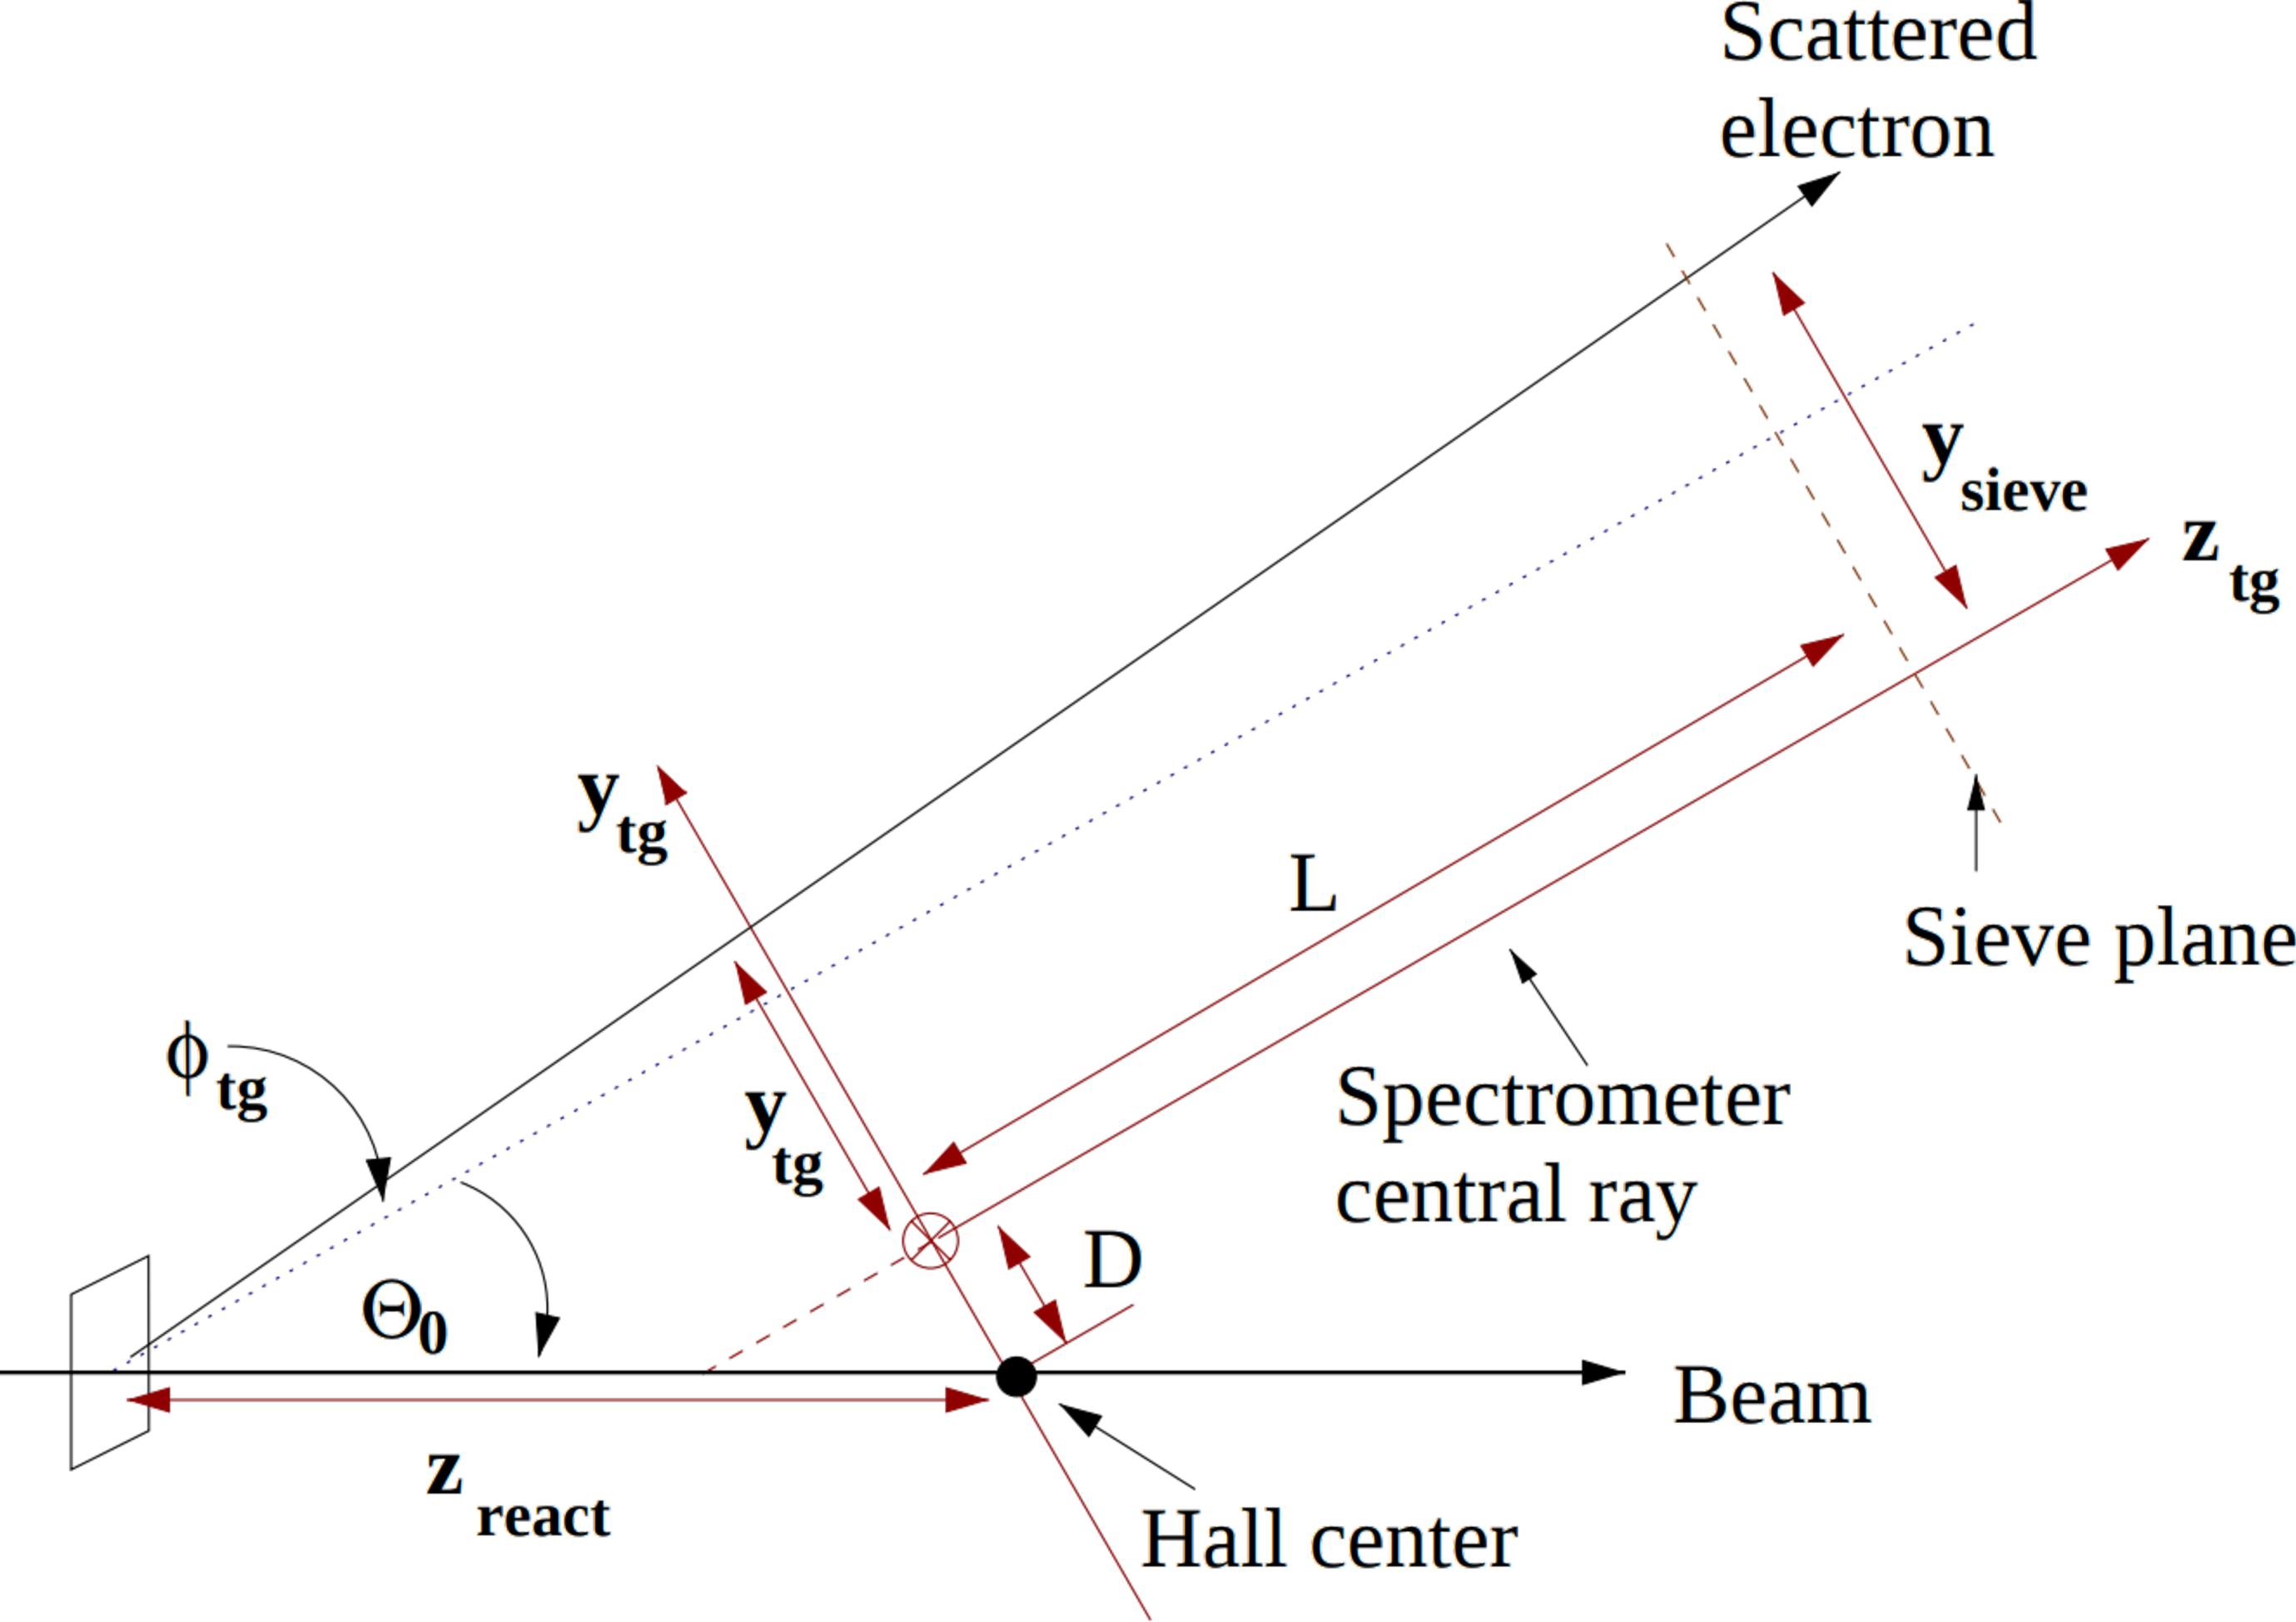
\includegraphics[width=11cm]{TCS.pdf}
		\caption{The TCS for an electron scattering event as seen from above. The event happens at $z_{react}$ distance from the Hall center. \textbf{L} is the distance from the Hall center to the sieve plane. \textbf{D} is the horizontal displacement of the spectrometer axis from the ideal position. $\Theta$ is the spectrometer's central angle \cite{optics}. }
		\label{fig:TCS}
	\end{figure}
	\item \textbf{Detector Coordinate System (DCS):}  The origin of the DCS is at the intersection of wire 184 of the U1 and V1 planes of the first VDC. $\hat{y}$ is parallel to the short symmetry axis of the lower VDC \cite{espace}. $\hat{z}$ is vertically up, perpendicular to the vdc planes.  $\hat{x}$  points away from the center of curvature of the dipole. The DCS values are calculated by using the intersection points of the 4 VDC planes and the spacial information of the VDC planes.
	\item \textbf{Transport Coordinate System (TRCS) at the focal plane:} Rotating the DCS clockwise around its y-axis by 45$^\circ$ generates the TRCS. The TRCS can be expressed by  DCS variables. 	
	\item \textbf{Focal Plane Coordinate System (FCS):} The FCS is used to transport an event's track from the DCS to the TCS. The FCS is determined by rotating the DCS around its y-axis by the angle between the local central ray and the $\hat{z}$ axis of the DCS. The local central ray is defined as a ray with $\theta = \phi =0$ for the corresponding relative momentum $\frac{\Delta_p}{p}$($\delta$) \cite{optics}. In the calculation of the FCS, the offsets of the VDCs are used to correct any misalignments.  
\end{itemize}
\paragraph{} The Analyzer provides two spatial coordinates and two angular coordinates for each event. These coordinates are determined by data received via the VDCs and decoded into the DCS. $x_{det}$ and $\theta_{det}$ is the particle's position and tangent of the angle made by its trajectory along the dispersive direction. $y_{det}$ and $\phi_{det}$ is the particle position and tangent of the angle perpendicular to the dispersive direction \cite{optics}. Using rotation matrices and other transfer definitions these DCS coordinates are converted to the FCS. The analyzer uses a calibration matrix to transport the FCS to the TCS. The first order approximation of the matrix can be defined as:
\begin{equation}
\begin{bmatrix}
	\delta \\
	\theta \\
	y      \\
	\phi   
\end{bmatrix}_{tg}
=
\begin{bmatrix}
	\langle \delta \vert x \rangle &\langle \delta \vert \theta \rangle & 0 & 0\\
	\langle \theta \vert x \rangle &\langle \theta \vert \theta \rangle & 0 & 0\\
	0 & 0 & \langle y \vert y \rangle &\langle y \vert \phi \rangle\\
	0 & 0 & \phi y \vert y \rangle &\langle \phi \vert \phi \rangle
\end{bmatrix}
\begin{bmatrix}
	x     \\    
	\theta \\
	y      \\
	\phi   
\end{bmatrix}_{fp}.
\end{equation}
The relationship between the focal plane variables and the target coordinates our conventionally expressed in a set of tensors, defined as Y$_{jkl}$, T$_{jkl}$, P$_{jkl}$, and D$_{jkl}$. These tensors are polynomials in x$_{fp}$ and are optimized to the 5th order. They can be use to relate the FCS to the TCS by the following relations:
\begin{align}
y_{tg} &= \sum_{j,k,l} Y_{jkl}\theta^j_{fp}y^k_{fp}\phi^l_{fp} \\
\theta_{tg} &= \sum_{j,k,l} T_{jkl}\theta^j_{fp}y^k_{fp}\phi^l_{fp} \\
\phi_{tg} &= \sum_{j,k,l} P_{jkl}\theta^j_{fp}y^k_{fp}\phi^l_{fp}  \\
\delta_{tg} &= \sum_{j,k,l} D_{jkl}\theta^j_{fp}y^k_{fp}\phi^l_{fp} 
\end{align}
The elements of the optics matrix used for the transporting from the FCS to the TCS are part of the tensors,Y$_{jkl}$, T$_{jkl}$, P$_{jkl}$, and D$_{jkl}$. The elements of the optics matrix are calculated via an optics calibration using a sieve slit and multi foil optics target. The procedure for calculating those matrix elements is in reference \cite{optics}. 
\paragraph{}Along with the tracking information in the TCS, the analyzer also provides the location of the reaction vertex, the scattering angle for the electron event, and the momentum of the scatted electron from the tracking information. The reaction vertex along the beam line, z$_{react}$, is the location where the scattering event happened in the HCS. z$_{react}$ can be found via the following relationship:
\begin{equation}
z_{react} = \frac{-(y_{tg} + \text{Spect\_Offset}_y) + x_{beam}(cos(\Theta_0) - \phi_{tg}sin(\Theta_0))} {cos(\Theta_0)\phi_{tg} + sin(\Theta_0)}
\end{equation}
The relationship for z$_{react}$ includes terms for the offset due to the mis-pointing of the spectrometer (Spect\_Offset$_y$), the offset of the beam at the point of intersection with the target (x$_{beam}$), and the setting for the spectrometer central angle ($\Theta_0$). The scattering angle of the electron, $\theta_{scat}$, is determined by a relationship wit the TCS angle coordinates $\theta_{tg}$ and $\phi_{tg}$ and the angle setting of the spectrometer. The relationship used to calculate the scattering angle from the target coordinates is described in reference \cite{HallA}, as:
\begin{equation}
\theta_{scat} = arccos \left( \frac{cos(\theta_{0})- \phi_{tg}sin(\theta_{0})} {\sqrt{1 + \theta_{tg}^2 + \phi_{tg}^2}} \right) \label{scatangle}
\end{equation}
The accuracy of the TCS angles $\theta_{tg}$ and $\phi_{tg}$ determine the accuracy of the measured scattered angle. The precise measurement of the scattering angle is crucial to every electron counting experiment. In order to provide accurate measurement of the scattering angle, a set of measurement surveys are completed. These surveys measure the:
\begin{itemize}
	\item the target position,
	\item the spectrometer central angle,
	\item the mispointing of the spectrometer nominal central ray from the hall center,
	\item the position of the sieve-slit center with respect to the nominal central ray,
	\item the position of the BPMs with respect to the ideal beam line \cite{HallA}.
\end{itemize} 
The results from the surveys have an approximate systematic uncertainty of 0.5 mm due to equipment uncertainties. The contribution of all the measurements uncertainties added in quadrature provide an approximate 0.6 mrad uncertainty to the overall measurement of the scattered angle \cite{HallA}. 
\paragraph{}The momentum of the scatted electron is also calculated via tracking information.  $\delta_{tg}$, the relative momentum of an event, is used in the calculation of the momentum of a particle traveling through the spectrometer. $p$, the absolute momentum for an event, is determine through, $p = p_0(1+\delta_{tg})$. $p_0$ is the central momentum setting of the spectrometer. This momentum setting of the spectrometer is determined via a measurement of the magnetic field ,B$_{dipole}$, of the HRS dipole. The determination of the central momentum from the magnetic field is given by a third order polynomial,
\begin{equation}
p_0 = \sum_{i=1}^{3} \Gamma_iB_0^i
\end{equation}
$\Gamma$ is a set of spectrometer constants calculated to an accuracy of $4\times10^{-4}$. The left HRS constants are $\Gamma_{1,2,3}$ (2702,0,-1.6), and the right HRS constants are $\Gamma_{1,2,3}$ (2698,0,-1.6) in units of MeV/T$^i$ \cite{HallA}. Once the analyzer produces a track for an event, the event can be included or excluded for future consideration. In the next section, I will discuses the selection of events for continued analysis.
 
\section{Electron Selection}\label{sec:ES}
\paragraph{} The extraction of the electron scattering cross section requires the counting of scatted electrons from a target. In order to count the number of scattered electrons, data is analyzed on an event by event basis. The event is passed through a number of criteria(cuts) in order to determine the identity and source of the scattered event. The cuts used for this analysis are separated into two different types, acceptance and particle identification(PID). The acceptance cuts are used to limit the source location and trajectory of the particle through the detector to provide greater accuracy for the reconstruction of the particle's scattered angle, momentum, and scattering vertex location. Cuts are also used to identify the particle and the type of scattering interaction it experienced. 
\subsection{Acceptance Cuts}
\paragraph{} The HRS was designed to accept particles within a range of $\delta$, $y_{tg}$, $\theta_{tg}$, $\phi_{tg}$, and the vertex location along the beam line. The acceptance of the spectrometer is well known near the central ray. Due to the geometry of the spectrometer's magnets, the distribution of accepted electrons at the edge of the acceptance is not well understood. This is shown in figure \ref{phi_comp}. Applying cuts in the target variables creates an area of acceptance that is well understood. The acceptance cuts used for this analysis are:

\begin{tabular}{@{$\bullet$ }lll}
-0.035 &$ >=$ &$\delta_{tg} <=$ -0.035\\
-0.04 rad &$>=$  &$\theta_{tg} <=$ -0.04 rad\\
-0.025 rad &$>=$  &$\phi_{tg}   <=$ -0.025 rad
\end{tabular}

\paragraph{}A cut is applied to the acceptance variable for the reaction location, Vertex z. The target cells are constructed of aluminum with thin end caps. Many electrons that are sent to the target scatter of the aluminum end caps. Figure \ref{EC5} shows distributions of the reaction vertex along the z axis of the beam line in the HCS for different gas filled cells and the empty cell. Comparing the empty cell to the cells filled with gas provides a observable comparison between the yield of events from the end caps of the cells to the yield of events from the gas in the cell. Figure \ref{EC5} also contains two vertical lines to demonstrate the locations of cuts selected to create the greatest area of acceptance of events from the target gas while also rejected most of the events from the end caps.   

\begin{tabular}{@{$\bullet$ }lll}
  -0.07 m &$>=$& Vertex Z $<=$ 0.09 m
\end{tabular}

\paragraph{} The analysis software assigns an event a track if the signal in the VDCs meet the required criteria. It is possible for the signal received by the VDC to produce multiple tracks for one event. Events that produce multiple tracks are cut out via a cut. These events are removed due the uncertainty of the correct track and position within the acceptance of the spectrometer. Section \ref{eff_track} contains a discussion of the efficiency of the cut applied to remove multi track events. 

\begin{tabular}{@{$\bullet$ }lll}
	Number of tracks == 0
\end{tabular}

\begin{figure}[]
	\centering
	\textbf{Spectrometer Acceptance}\par\medskip
	\vspace*{-5pt}
	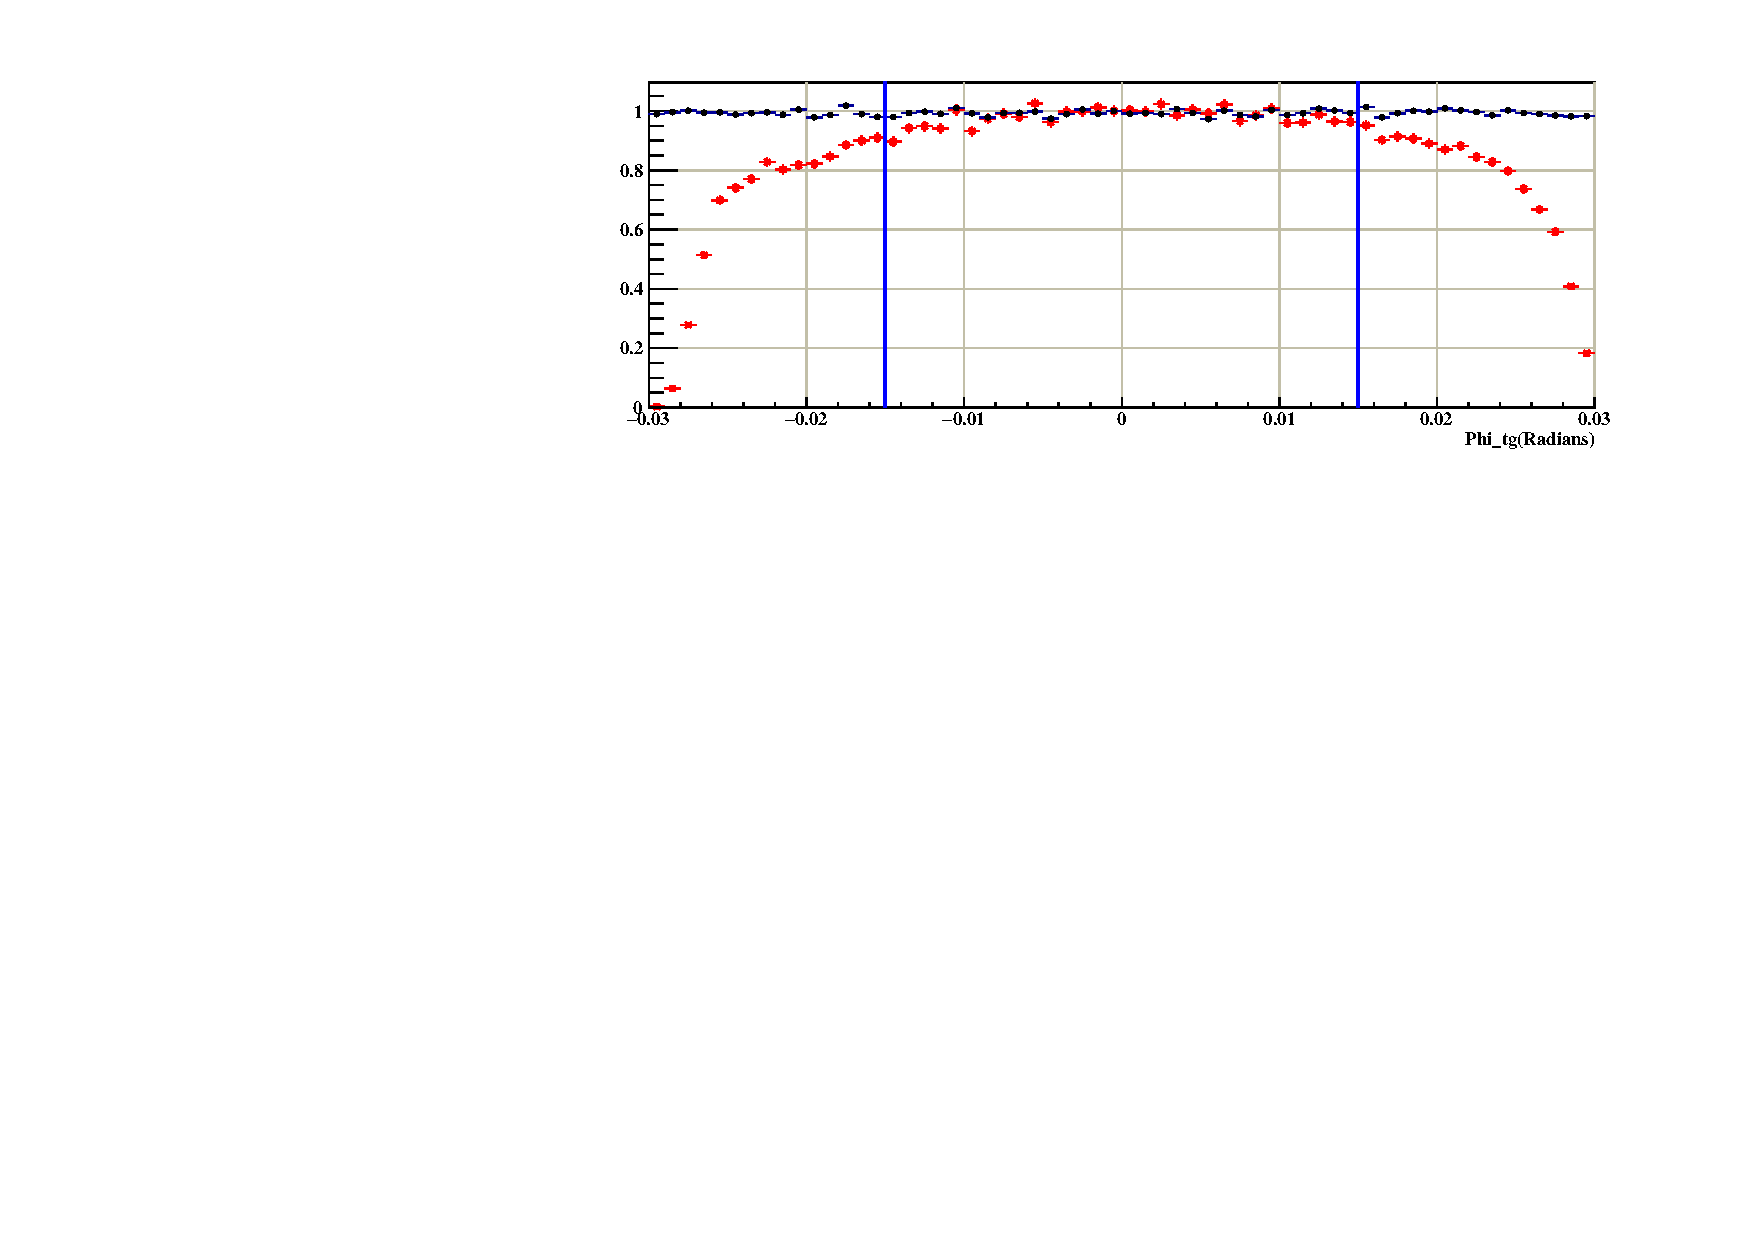
\includegraphics[width=15cm]{Phi_tg_comp_1.pdf}
	\caption{Simulation of events to demonstrate the acceptance of the spectrometer. Black events have been generated with no acceptance effects, Red points include a cut to only allow events that transverse the entire spectrometer. The Blue lines are example locations of cuts used in event selection to exclude the edge of the acceptance. }
	\label{phi_comp}
\end{figure}


\subsection{Identification Cuts}
\paragraph{} The process of capturing data from the two HRSs begins with the firing of a trigger. The trigger design for MARATHON focused on triggering for electrons and reducing the amount of other particles. Figure \ref{fig:trig_layout} describes the design of MARATHON's main trigger and efficiency triggers. MARATHON's main trigger, trigger 2, consist of a $(So \& S2) \& GC$. This was discussed in section \ref{sec:Trig}. Using the scintillators as a trigger allows the capture of data from charged particles that pass through the detector. These particles are mainly electrons and pions. The addition of the GC to the trigger allows for a first pass cut on unwanted particles. Applying a MARATHON trigger cut to the data narrows the sample of non-electrons that need to be analyzed. The trigger data is stored bitwise by the analysis software to allow for the capture of every trigger that fired for the event. The trigger cut applied for this analysis requires the event to fire the MARATHON trigger but does not exclude events that fire multiple triggers. This is accomplished by bitwise comparing the trigger to 1 bit shifted to the left by 2.  
   
\begin{tabular}{@{$\bullet$ }lll}
	MARATHON trigger (bit) &\& &(1$<<$2)
\end{tabular}

\paragraph{}One of the largest sources of contamination for the MARATHON experiment are negatively charged pions. These pions are removed through software cuts made in the total signal from the ten cherenkov PMTs(photomultiplier tubes) and the energy deposited into the blocks of both layers of the calorimeter. Electrons can be identified by their behavior in the spectrometer. High-quality electrons will track through the entire detector stack to deposit most of their energy into the total calorimeter system and creating a large amount of light in the cherenkov. An efficiency scan is used to determine the best location for the cuts in the calorimeters and cherenkov. A efficiency scan for the two layers of the calorimeters is shown in figure \ref{cal_pidscan}. The scan covers a large range of possible energy deposition in a layer of the calorimeter calculating both the efficiency of rejecting pions and of counting electrons. The description of how the efficiency is calculated can be found in section \ref{ss:PID}.

\begin{tabular}{@{$\bullet$ }lll}
	Total Cherenkov adc sum &$>$ &1800\\
	Calo. Layer 1 Energy &$>$ & 1 GeV\\
	Calo. Layer 2 Energy &$>$ & 0.6 GeV
\end{tabular}

\begin{figure}[]
	\centering
	\textbf{PID Cut Scan }\par\medskip
	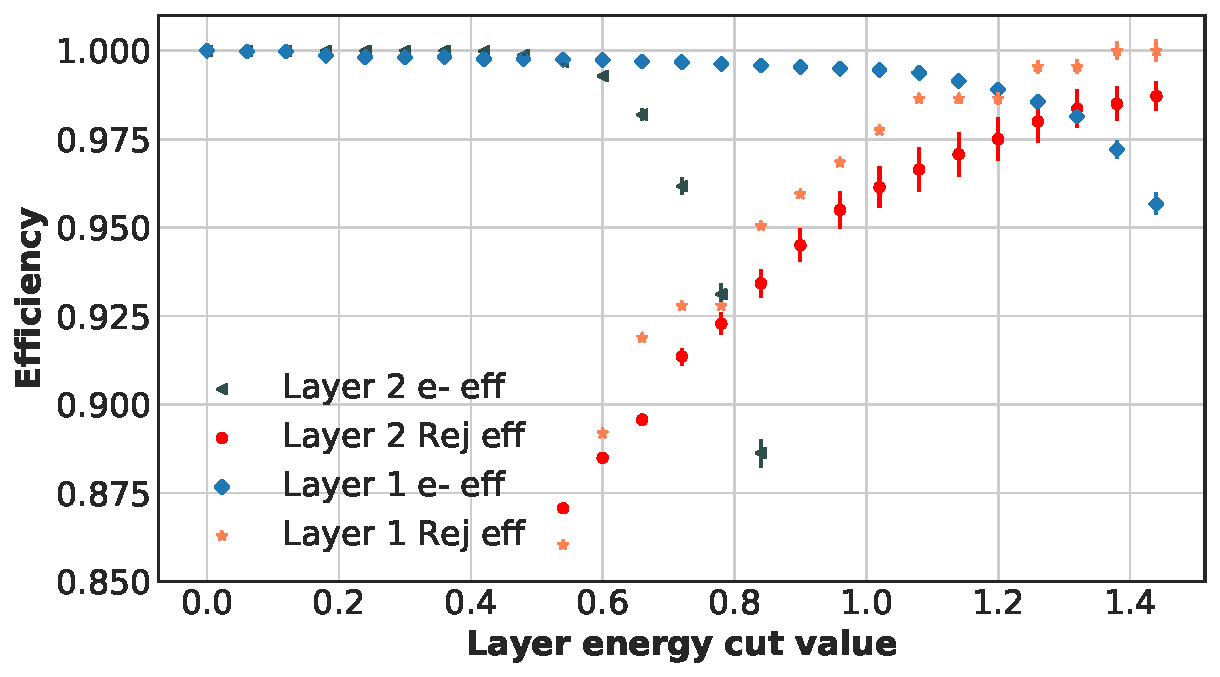
\includegraphics[width=13cm]{PID_3layer_plot.pdf}
	\caption{ A scan of the PID efficiency for a cut in each layer of the calorimeters.}
	\label{cal_pidscan}
\end{figure}

\paragraph{}The electrons that have pass all of the previous discussed cuts are tools used to study the scattering interaction and the components of the scattering interaction that produced the resulting event. The kinematics used for the MARATHON will produce events in the DIS, resonance, and quasi-elastic regimes of the scattering spectrum. A cut is applied to the invariant mass of the scattered event to only include events that are deeply inelastic. 

\begin{tabular}{@{$\bullet$ }lll}
	W$^2$ &$>$ &2.5\\
\end{tabular}

\paragraph{}Events that pass all the criteria discussed in this section are considered to be a good electron and will be counted for the extraction of the cross section. 
%cuts, total electrons per kinematic, binning in x 

\section{Efficiencies}\label{effs}
\paragraph{}The high resolution spectrometers are capable of detecting a myriad of particles that track through the detectors. The design of an experimental trigger uses the properties of the individual detectors to capture data of meaningful events. Many accidentals, background, and unwanted events trigger the data acquisition system, and some good electrons are missed by our DAQ. The removal of these unwanted events takes place during analysis via software cuts. Restricting the applicable signal from certain detectors through different cuts allows for the rejection of background particles and prevents contamination in the yield extraction. The efficiency of the HRSs and the software cuts applied will be discussed in this section.  

\subsection{Computer and electronic Livetime}
\paragraph{}The signal from events that fire the DAQ travel through electronics like amplifiers and logic modules on its way to be recorded by the TDCs and ADCs. The processing of these signals require time at each stage. During that time another event will be discarded due to limitations in the hardware. This time when the DAQ system cannot handle another event is known as the dead-time of the system. livetime therefor is the percentage of time when an event can be recorded. The lost events need to be account for during the analysis process. The livetime of the DAQ system for the MARATHON experiment was measured by determining the percentage of events that were recorded relative to the number of events that fired the corresponding trigger. The livetime for the MARATHON experiment depended on the rate of events. The livetime during the highest rate kinematic was determine to be 0.947, and climbs to 0.998 for the highest angle setting. Listed in table \ref{LTtable} are the calculated values for livetime at each kinematic. 

\begin{table}[]
	\textbf{Livetime for each kinematic }\par\medskip
	\begin{tabular}{|l|l|l|l|l|l|l|l|l|l|l|}
		\hline
		Kin      & 1 & 2 & 3 & 4 & 5 & 7 & 9 & 11 & 13 & 15 \\ \hline
		LiveTime & 0.947 & 0.969 & 0.981 & 0.986 & 0.992 & 0.996 & 0.997 & 0.998  & 0.998  & 0.998\\ \hline
	\end{tabular}
	\caption{Livetime during the MARATHON experiment calculated using trigger 2.  }
	\label{LTtable}
\end{table}
  

\subsection{Particle Identification Efficiency}\label{ss:PID}
\paragraph{} The contamination of pions is a large concern for the counting of scattering electrons. Software cuts are used to remove the pions from the electron count. The efficiency of the PID cuts will be discussed in this section. Plotting the signal in the cherenkov versus the energy deposited into both layers of the calorimeter allows for visual representation of the sampling cuts made in the efficiency studies, which can be seen in figure \ref{elesample}. 
\begin{equation}\label{effequ}
\begin{split}
GE_{sample} & = \textrm{Known electron sample from tight cut}  \\
GE_{pass} & = \textrm{$GE_{sample}$ and pass indentification cut} \\
Electron_{eff}  & = \frac{ GE_{pass} } { GE_{sample} } 
\end{split}
\end{equation}
\begin{figure}[]
	\centering
	\textbf{Cherenkov sum versus Total Energy deposited }\par\medskip
	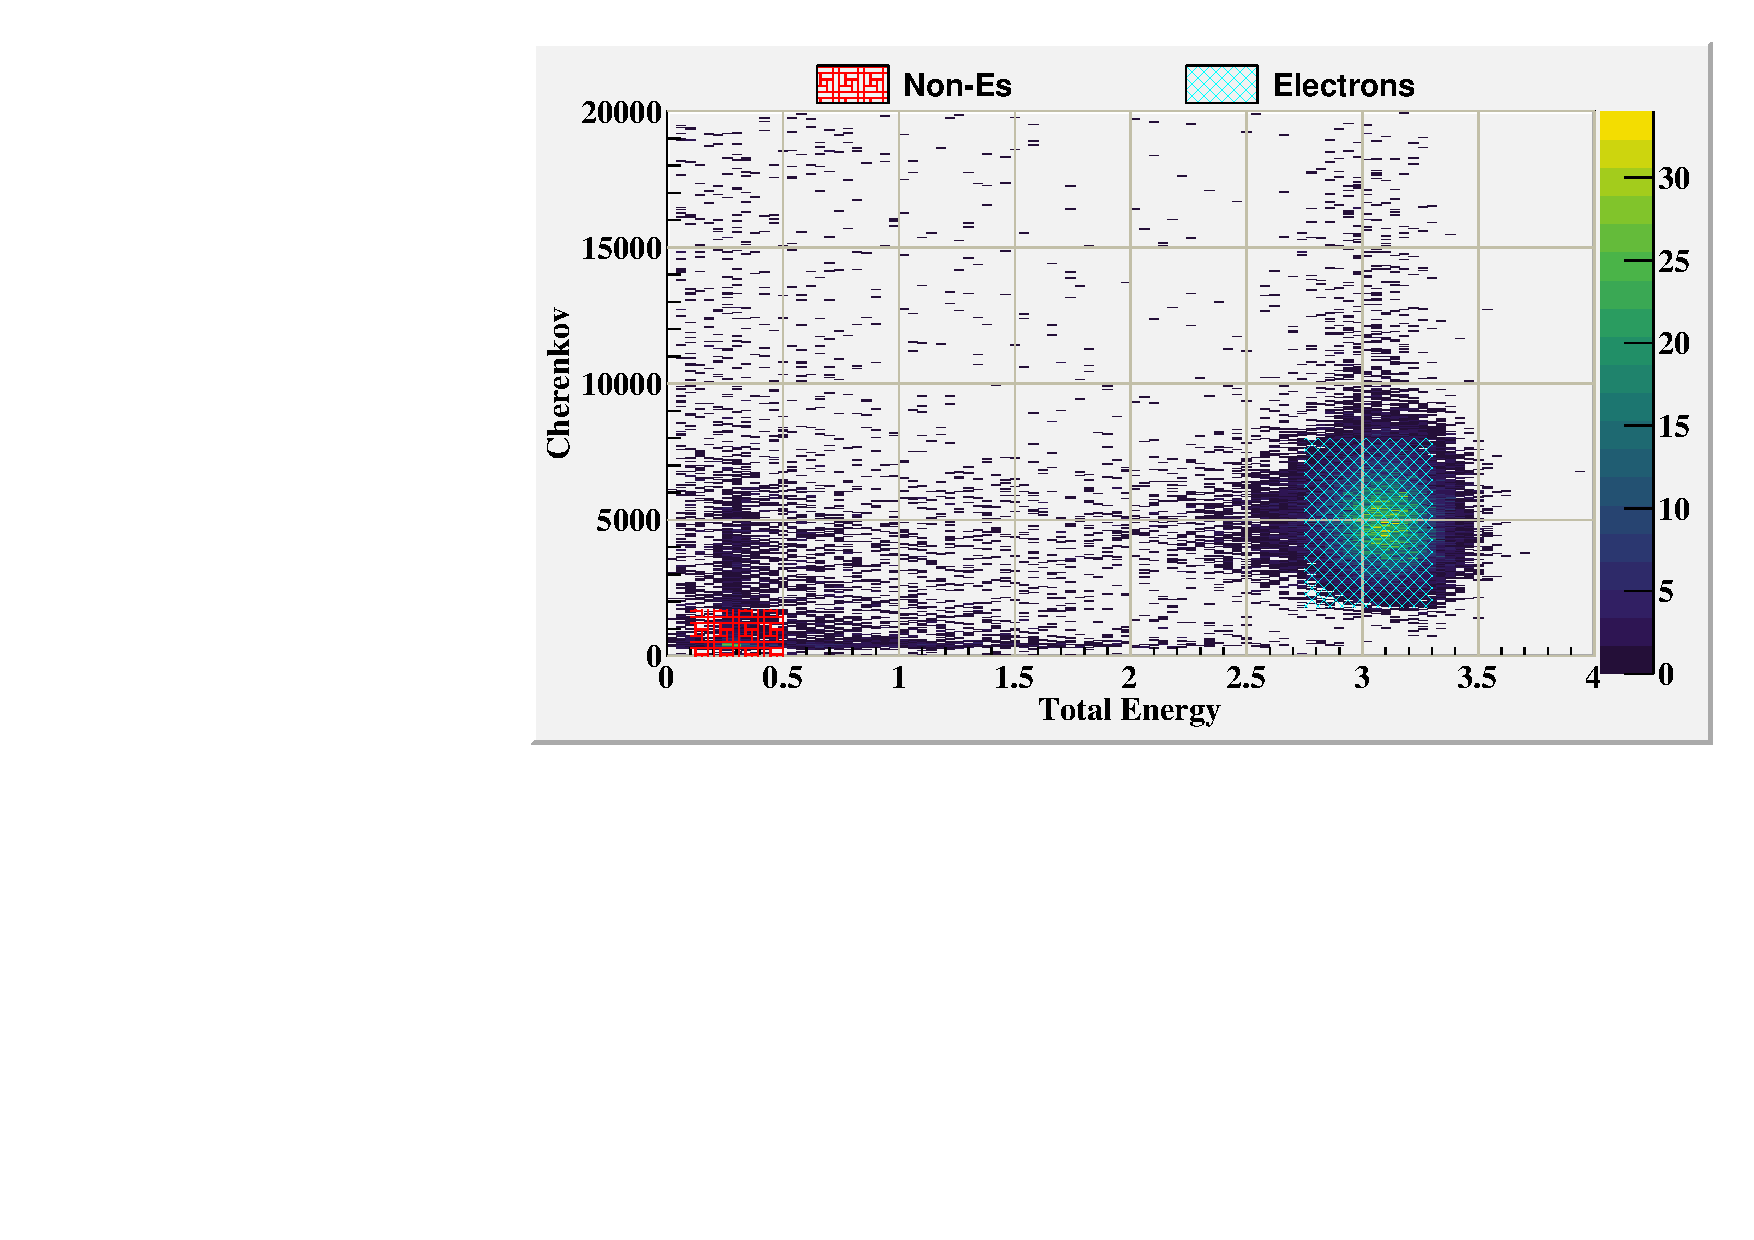
\includegraphics[width=13cm]{PID_2d}
	\caption{Two dimensional plot of the cherenkov sum versus Total Energy deposited, including electron sampling in teal and non-electron sampling in red. }
	\label{elesample}
\end{figure}

\begin{figure}[t]%
	{\centering
		\textbf{Particle ID and efficiency sampling for PID detectors }\par\medskip}
	\centering
	\subfloat[]{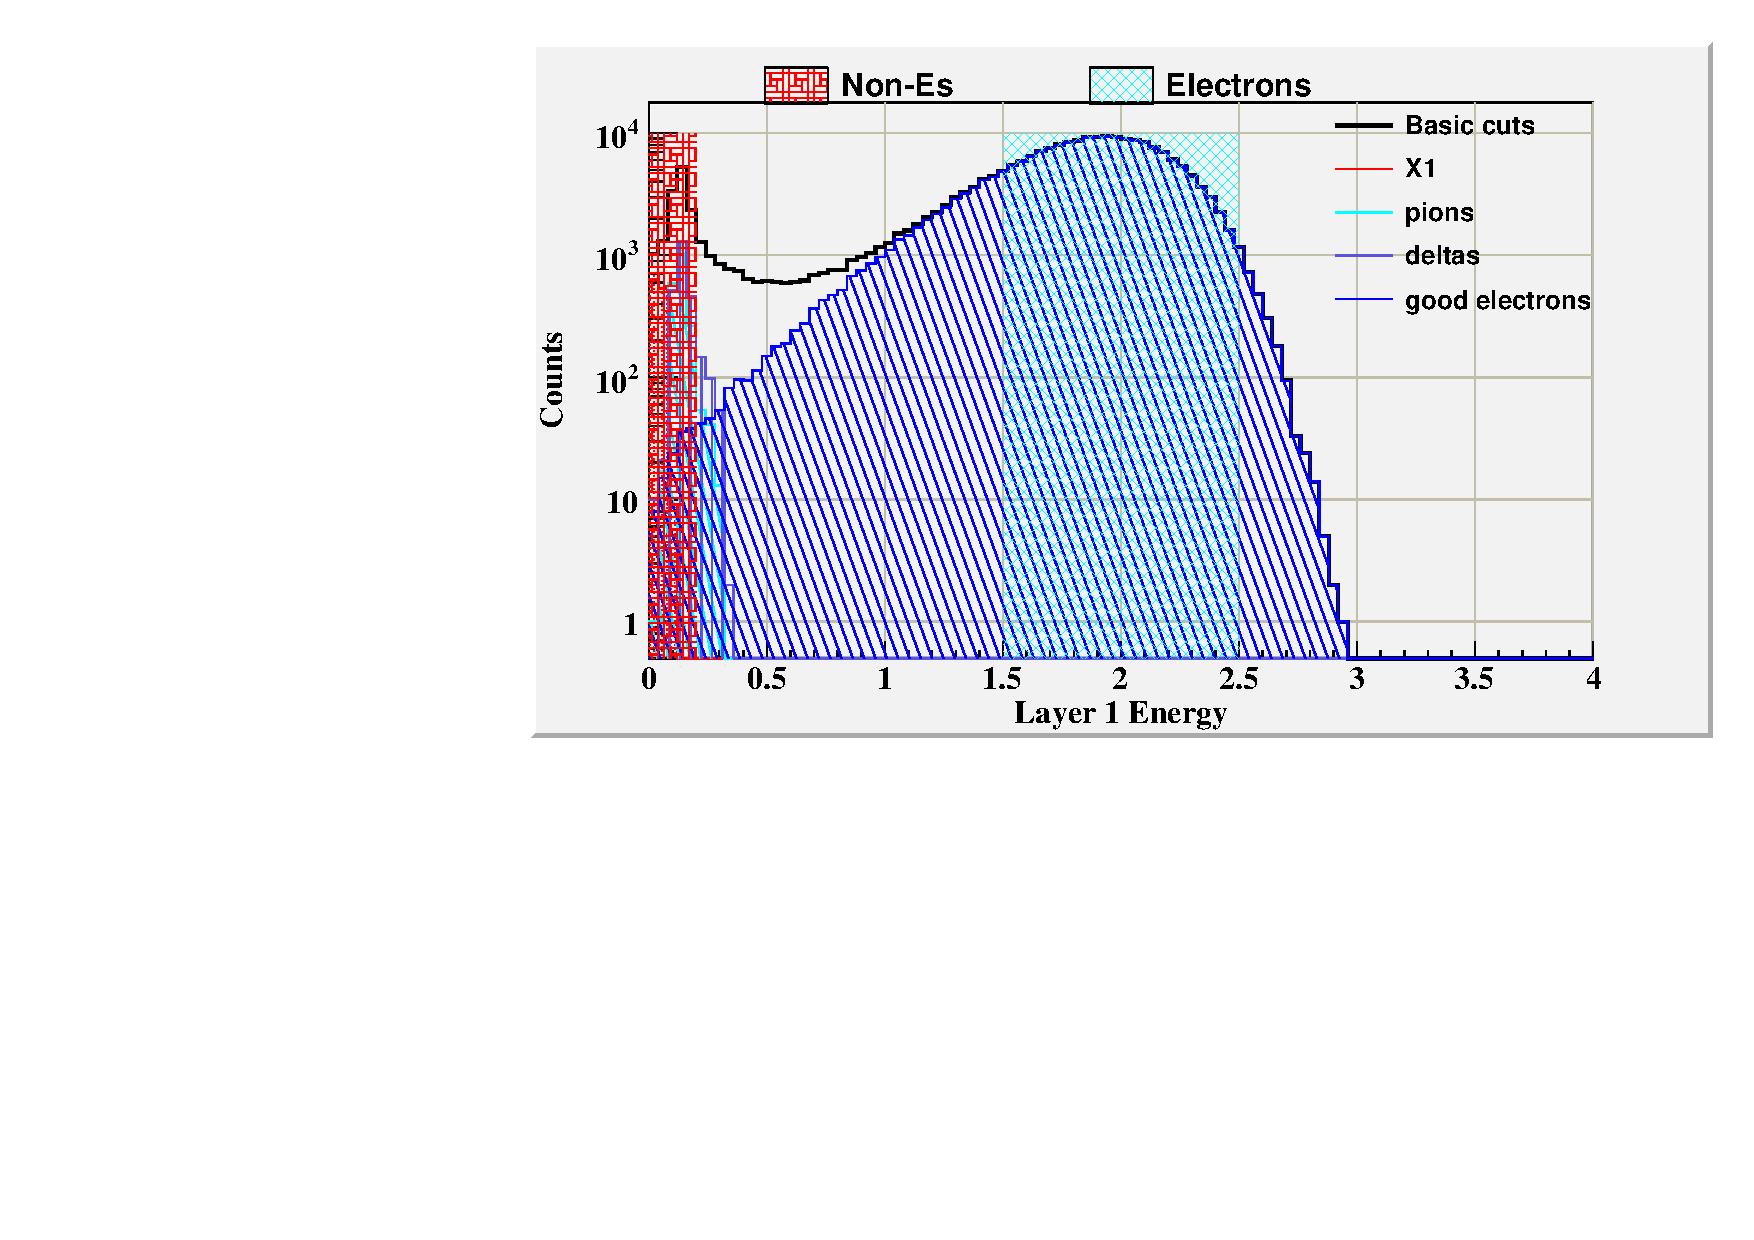
\includegraphics[width=0.5\textwidth,height=4.5cm]{Lprl1}\label{samA}}%
	\subfloat[]{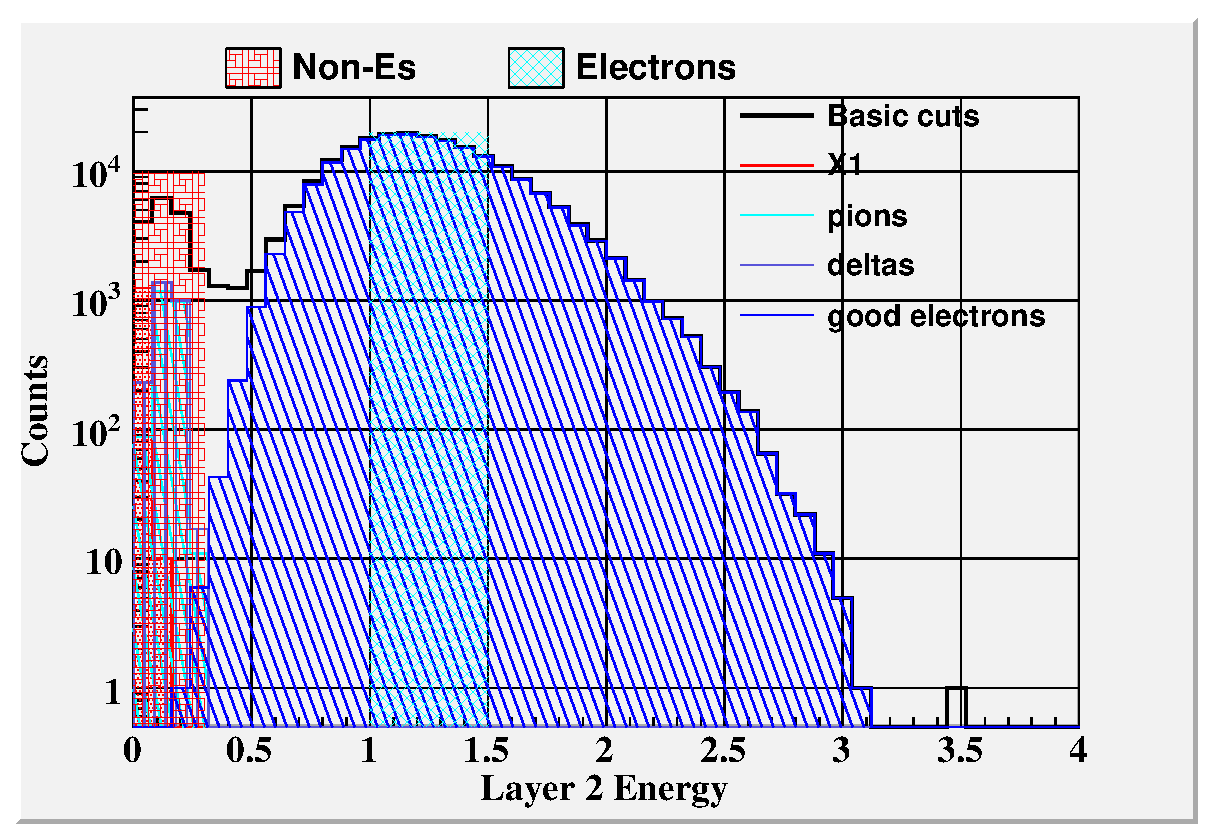
\includegraphics[width=0.5\textwidth,height=4.5cm]{Lprl2}\label{samB}}\\
	\subfloat[]{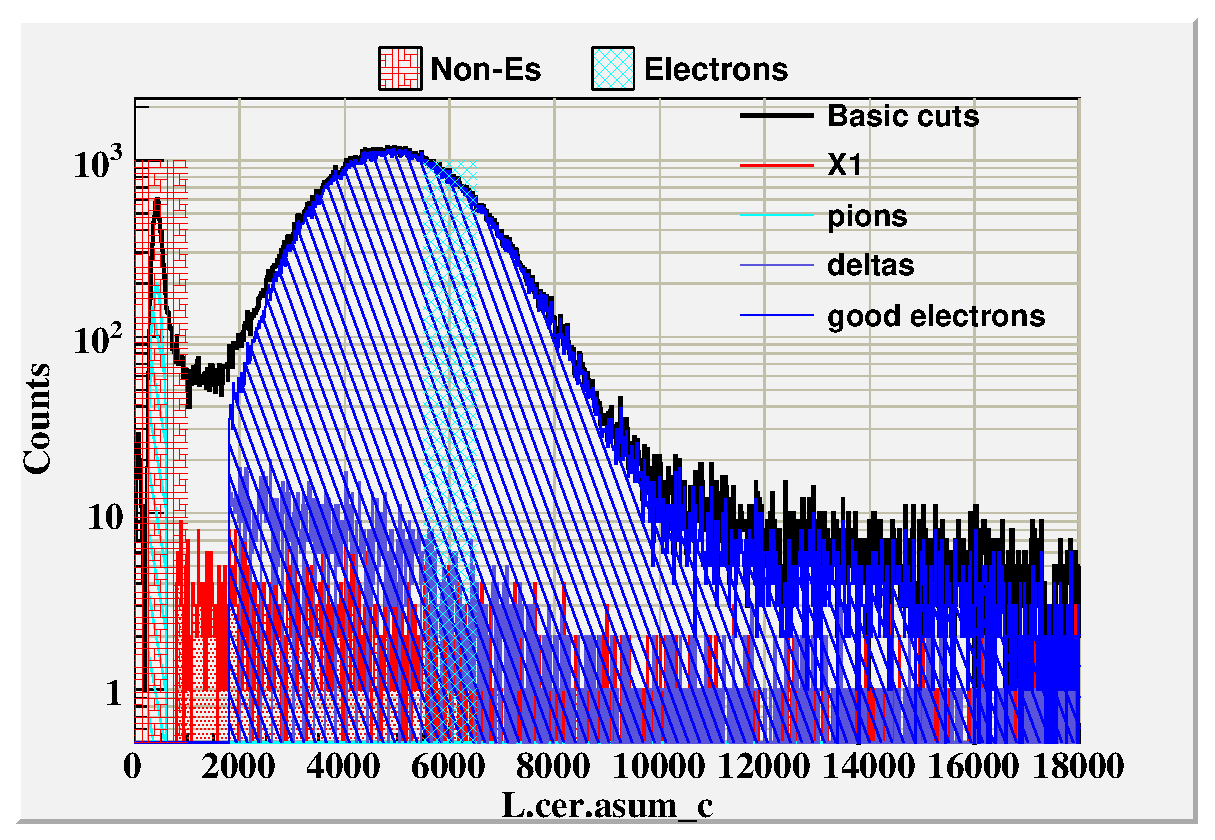
\includegraphics[width=0.95\textwidth,height=3.85cm]{Lcerasum}\label{samC}}%
	\caption{Electrons and other back ground particles identified via cuts in the total calorimeter and the gas cherenkov shown in the individual layers of the calorimeters and the cherenkov. Sampling cuts for Electrons in teal and Non-Electrons in red.}%
	\label{sampling}%
\end{figure}


\paragraph{}The efficiencies of the spectrometer's particle identification(PID) detectors were determined by using the first calorimeter layer, the second calorimeter layer, and the cherenkov to provide samples of good electrons and other particles. The PID efficiency of the individual detectors was determined using equation \ref{effequ}. The good electron sample for calculating the efficiency of the single detector was defined by sampling through the other two detectors. Sampling through the two layers of the calorimeter is shown in figure \ref{samA} for the first layer of the calorimeter and \ref{samB} for the second layer. The cherenkov good electron sample is shown in figure \ref{samC}. The electron sample from the cherenkov is contaminated by delta rays and a combination of unknown particles. These unidentified background particles are known to be relativistic due to the amount of light seen in the cherenkov. However, the events do not deposit enough energy into the calorimeter system to be considered as a good electron that scatter from our target through the detector. Using sampling in one layer of the calorimeter and the cherenkov, these unwanted low energy particles are rejected from sampling for efficiency calculations. The electron selection PID efficiency for the three PID detectors was determine at each kinematic setting to be approximately 98$\%$ . The efficiency was determined to be independent of the kinematic setting. Only small fluctuations were seen during the study, these small changes are due to decrease in statics, and all of the results fall within statical uncertainty of being independent of kinematic setting. The non-electron suppression efficiency was determine as part of this PID efficiency study to ascertain how many back ground particles leak into our sample of good electrons after cuts our made. The suppression efficiency of the cherenkov suffered due to the contamination of the relativistic low energy particles. Combining the two calorimeter detectors with the cherenkov increased the overall suppression efficiency for the spectrometer to 99.9$\%$ over the entire kinematic range of the MARATHON experiment. 

\begin{figure}[t]
	{\centering
		\textbf{PID efficency for each detector for all kinematics. }\par\medskip}
	\centering
	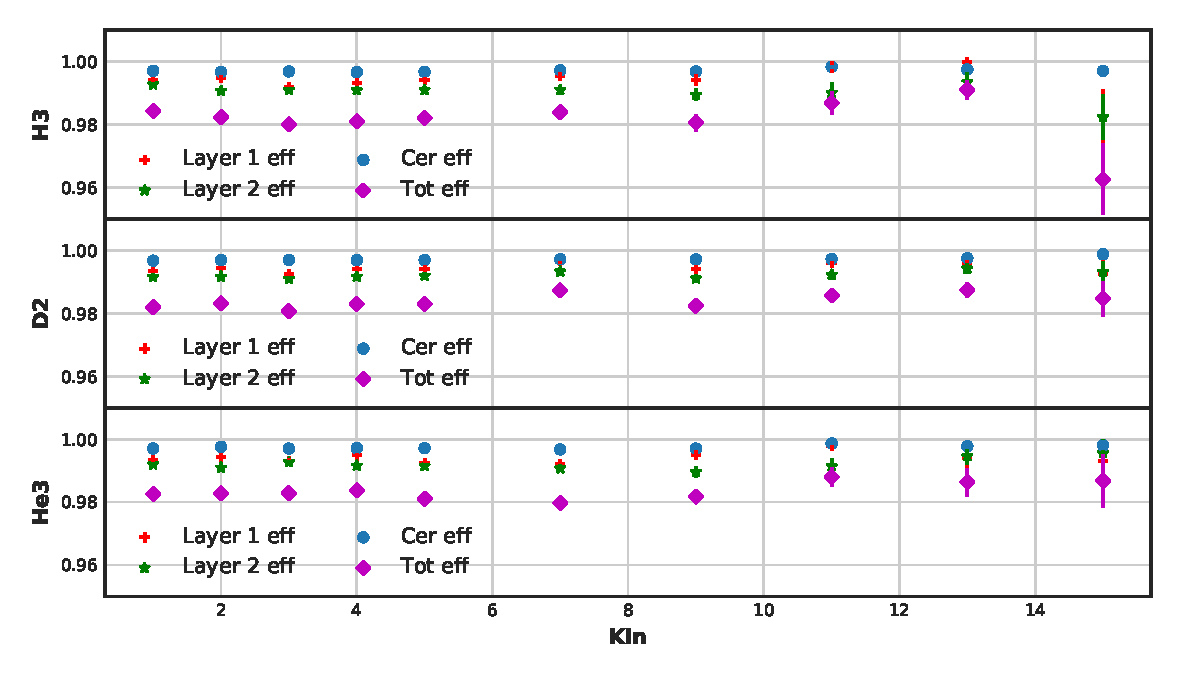
\includegraphics[width=15cm]{PID_allkin_alltgt}
	\caption{The PID efficiency for the cherenkov and both layers of the calorimeter,including the overall total PID efficiency for each of the gas targets at all of the kinematics.}
\end{figure}

\subsection{Trigger Efficiency}
\paragraph{}  Due to inefficiencies of the electronics, logic, and detectors an event can produce a false trigger or a high quality electron may not fire the main trigger.
\begin{figure}[]
	\centering
	\textbf{Trigger efficiency for the MARATHON experiment }\par\medskip
	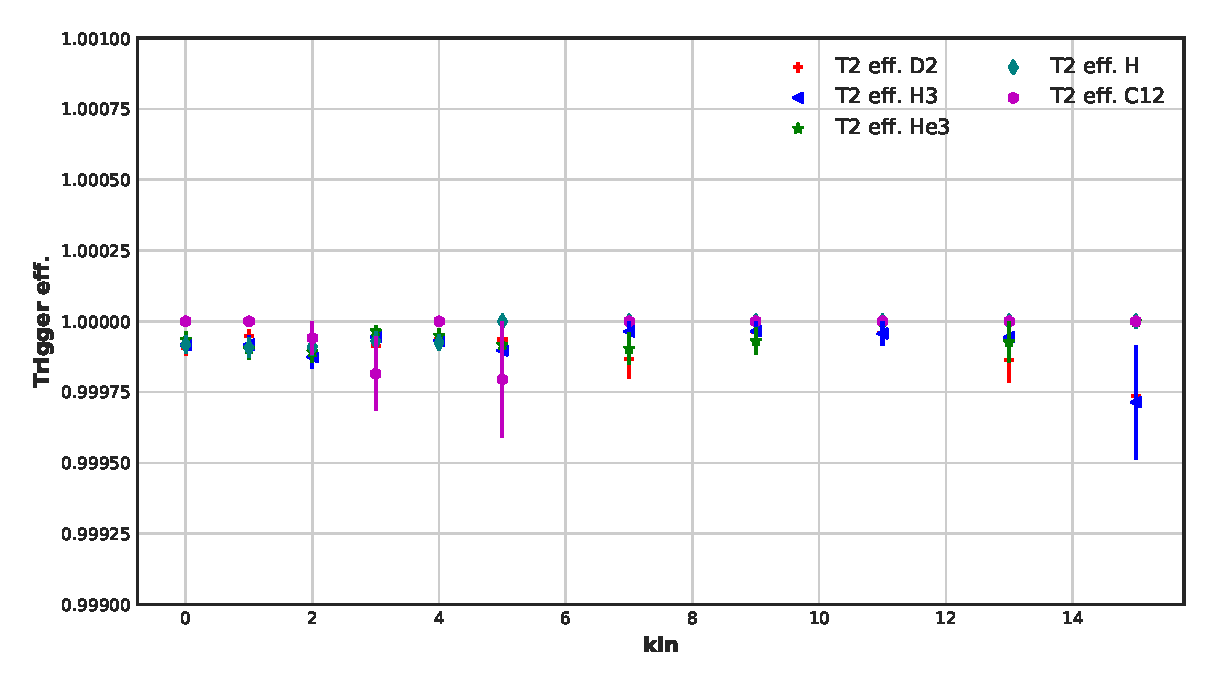
\includegraphics[width=14cm]{Trigger_Eff.eps}
	\caption{Trigger efficiency of trigger 2 for different targets at all kinematics calculated via sampling from trigger 1. }
	\label{trigeff}
\end{figure}
A low threshold in the cherenkov signal allows for an inclusive trigger limiting the overall number of quality electrons missed, but allows for a large quantity of none-electron triggers. Software PID cuts prevent the contamination of non-electrons in the yield calculation. The tight PID software cuts removes the false positive inefficiency from the trigger design and is then considered in the PID efficiencies. The trigger inefficiency caused by missed high quality electrons was then calculated by sampling the high quality electrons in trigger 1, $(S_o \& S_2)$. This ties the efficiency of trigger 2 with the performance of the scintillators. The efficiency of the two scintillating planes in conjunction is calculated by using sampling in trigger 3, $(S_o | S_2) \& Cer$ with strict PID cuts in both layers of the calorimeters and requiring a hit in the cherenkov. The two scintillator planes in conjunction have an efficiency greater than $99.7 \% $ for all kinematics. Combining the trigger efficiency of the main trigger shown in figure \ref{trigeff} with the performance of the scintillators give an over all efficiency for the trigger of the MARATHON experiment of greater then $99.6\%$.

\subsection{Tracking Efficiency}\label{eff_track}
\begin{figure}[]
	\centering
	\textbf{Tracking efficiency for the MARATHON experiment }\par\medskip
	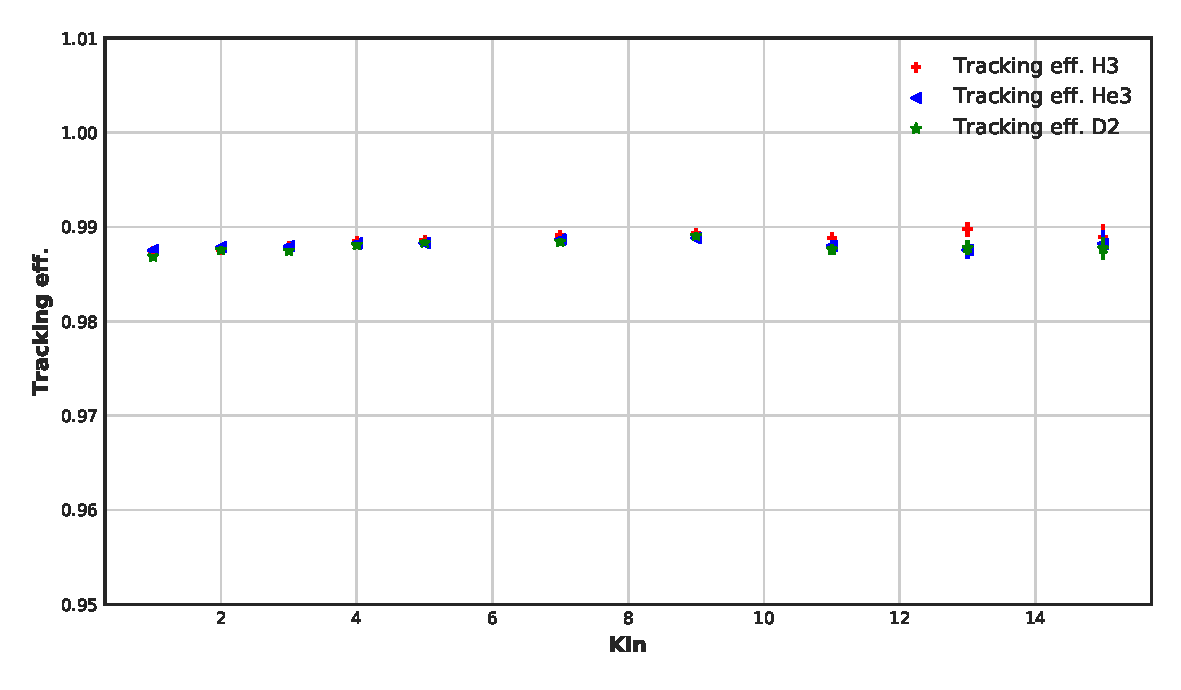
\includegraphics[width=15cm]{Tracking_Eff_allkin.eps}
	\caption{Tracking efficiency of the VDCs for different targets at all kinematics. }
	\label{trackeff}
\end{figure}
\paragraph{}Particles that travel through our detector could originated from sources wanted or unwanted. In order to control the source of the scatter electrons, we use a particle's track to identify its source. The signals received via the VDC is used to produce a particles track from the target to end of the spectrometer. The largest source of inefficiency for the VDCs are incorrectly identified tracks. High quality electrons that transverse the spectrometer should only have one good track, calculated via the tracking package in the analysis software. The capability of the VDCs to determine a good electron event's one good track is know as the one track efficiency for the VDCs. Quantitatively the one track efficiency ($\epsilon_{VDC}$) can be obtained via:
\begin{equation}
\epsilon_{VDC} \equiv \frac{N_{1 track} }{N_{all}}
\end{equation}
Where the number of good electron events that have one good track is defined as $N_{1 track}$, and $N_{all}$ are all of the electrons rather they have a good track or not. The good electron selection is made via PID cuts in the calorimeter and cherenkov, and cuts in the ADC and TDC of the scintillators. Direct cuts in the signal of the scintillators where made to include the nominal acceptance cuts, which our produced through tracking software. The tracking efficiency of HRSs during the MARATHON experiment is shown in figure \ref{trackeff} for the three gas targets during all kinematic ranges. The efficiency of the VDCs is not relative to the angle of the spectrometer. So the uniform tracking efficiency across all kinematics is expected and helps eliminate any concerns of the performance of the VDCs during the experiment. 

\section{Background Subtraction}
\paragraph{} The purpose of this analysis is to study the DIS cross sections of deuterium, helium-3, and tritium. The sample of scattered events used to determine the cross section of a given nuclear target then needs to be cleaned of any contamination produced from other targets and processes. The electrons detected by the spectrometers can be electrons that scatted from our chosen target, scattered from a source other then our target, or produced through process other than DIS scattering. The two sources of contamination for the MARATHON experiment are events scattered from the aluminum end caps of the target cell and pair produced electrons via photon interaction. The tritium gas will experience beta decay, that produces helium-3. This helium-3 that contaminates the tritium cell will also be addressed in this section.
\subsection{End Caps}
\paragraph{} The target cells used during the MARATHON experiment are shown in figure \ref{HATT}. The majority of the events from the end caps can be removed easily via a cut in the reconstructed quantity of reaction vertex along the beam axis. The relatively large density thickness of the aluminum end caps cause a large amount of end cap contamination. The majority of the electrons that scatter from the end caps can be removed through software cuts in the reaction vertex along the beam axis(z). Show in figure \ref{EC5} is a comparison of the reaction vertex of the electron events between the gaseous targets and the empty cell target at kinematic 4. The yield is normalized by the number of event in the histogram to remove any bias from the amount of time of beam on target. The empty target  results in figure \ref{EC5}, demonstrate the form of scattering off of the aluminum windows of our target cell. Using the reconstructed vertex location of the scattering origin, the vast majority of the events from the windows can be removed. This vertex cut is shown by the two vertical blue lines. Only events that lie within these two line are considered good electrons from our chosen target. 


\begin{figure}[]
	\centering
	\textbf{Scattering vertex along the beam axis. }\par\medskip
	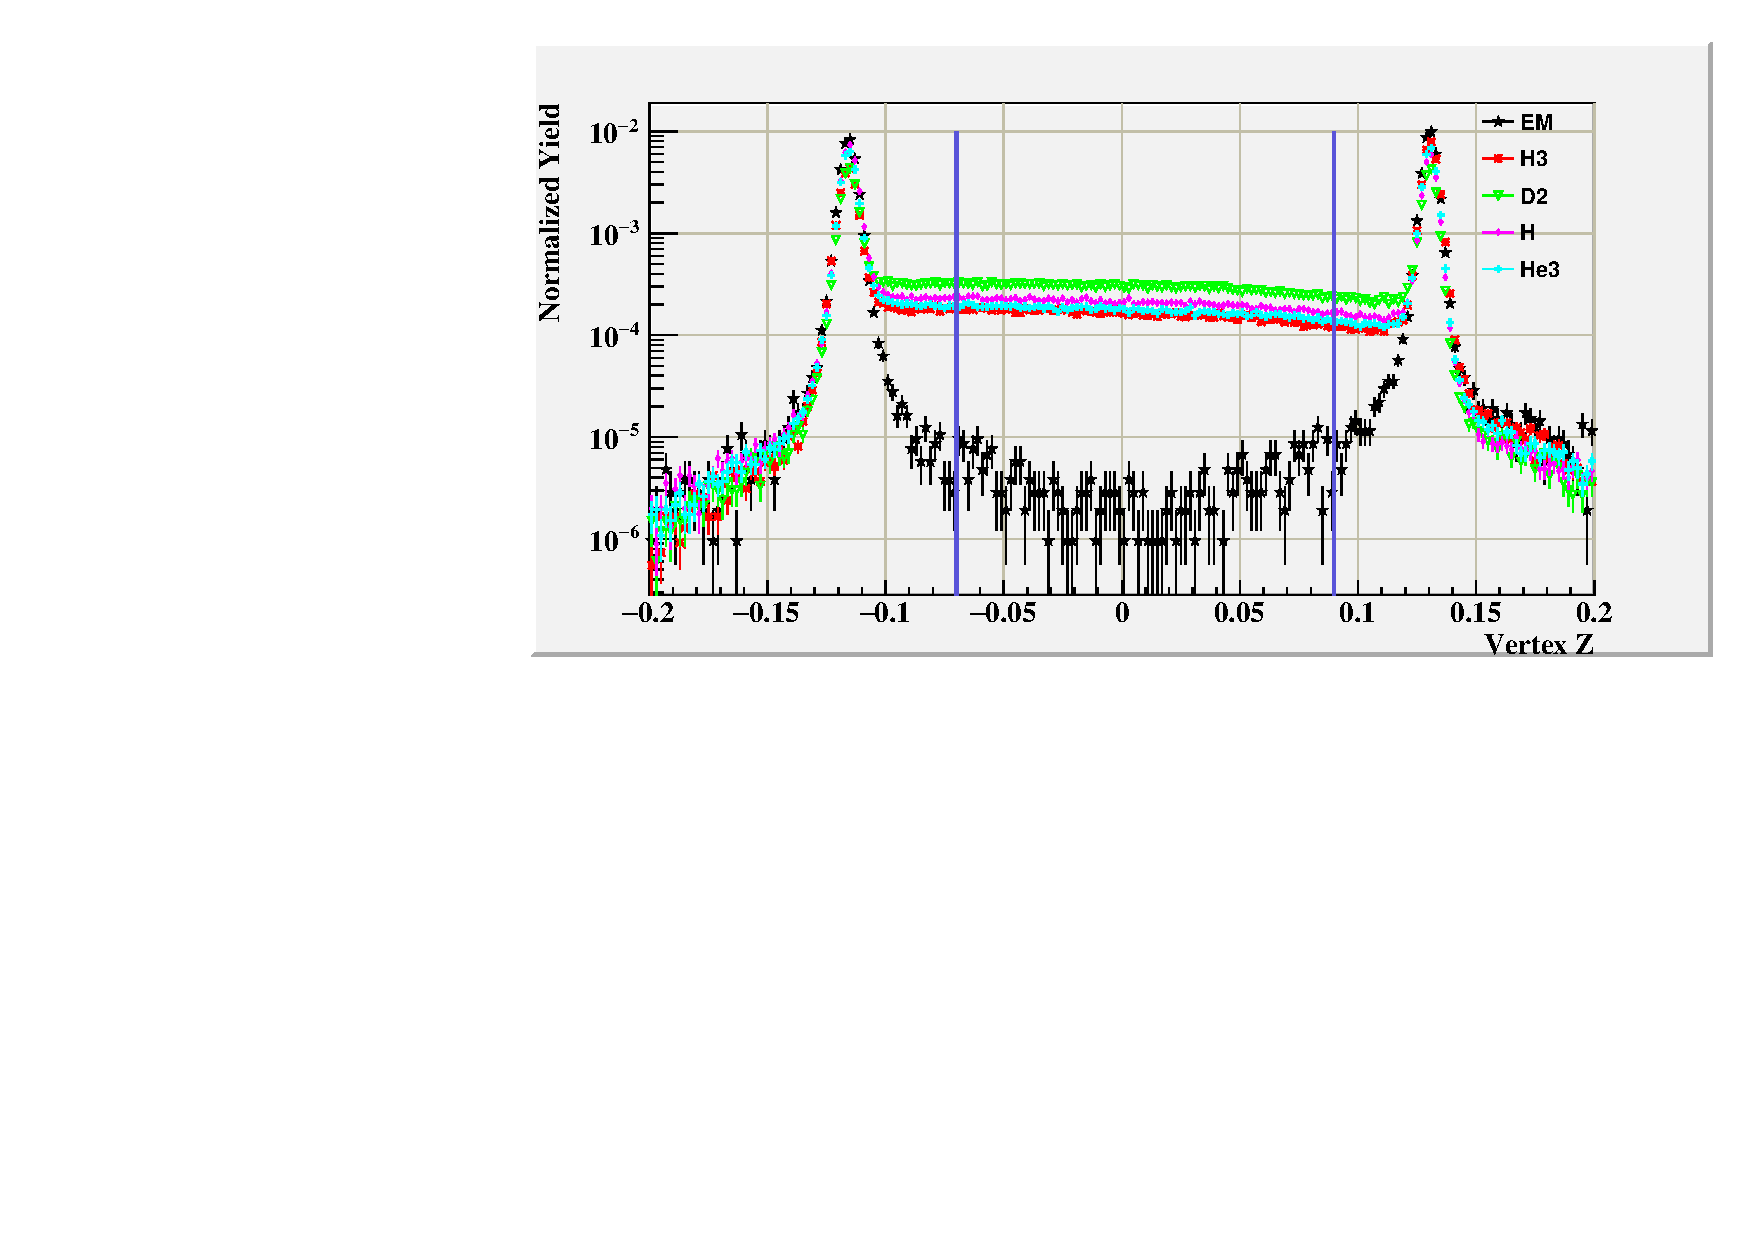
\includegraphics[width=15cm]{endcap_kin4.pdf}
	\caption{Comparison of the scattering vertex along the z axis for the empty target(EM) and the gas targets at kin. 4. }
	\label{EC5}
\end{figure}

\paragraph{}The empty cell vertex z disruption does have content within the vertex cut. These events that remain after the cut are corrected for via an end cap contamination factor. This  factor is calculated by determining the ratio of the number of good electrons that scatter from the empty cell and from each gas cells, resulting in ratio of $\big(\frac{Yield_{EC}}{(Yield_{Gas} + Yield_{EC})}\big)$. Where the subscript EC denotes events from the end caps. The correction factor applied to the yield calculation is defined as:
\begin{equation*}
ECC = 1- \big(\frac{Yield_{EC}}{(Yield_{Gas} + Yield_{EC})}\big) \equiv \frac{Yield_{gas}}{(Yield_{Gas} + Yield_{EC})}
\end{equation*}

%\begin{table}[]
%	\textbf{End cap contamination for each target at all kinematics. }\par\medskip
%	\hspace{-70pt}
%	\begin{tabular}{|l|l|l|l|l|l|l|l|l|l|l|}
%		\hline
%		Kinematic  & 1       & 2       & 3        & 4        & 5        & 7       & 9       & 11       & 13       & 15   \\ \hline
%		H3   & 0.0218 & 0.0202 & 0.0163   & 0.0154   & 0.01445  & 0.01177 & 0.009   & 0.0069   & 0.0055   & 0.0043     \\ \hline
%		He3  & 0.0251 & 0.0229 & 0.01839  & 0.01727  & 0.01573 & 0.0125  & 0.00974 & 0.00715  & 0.00572 & 0.00449  \\ \hline
%		D2   & 0.0113 & 0.010  & 0.008206 & 0.00934 & 0.00864  & 0.00831 & 0.0057  & 0.00512 & 0.00379  & 0.00276   \\ \hline
%		H    & 0.0238  & 0.020 & 0.0178   & 0.0176   &          &         &         &          &          &            \\ \hline
%	\end{tabular}
%	\caption{The amount of electrons that scatter from the empty cell compared with the amount electrons that scatter off a gas filled cell. }
%	\label{ECCtable}
%\end{table}



\subsection{Pair Produced Electrons}
\paragraph{} The high energy scattering interaction used to create deep inelastic scattering events can produce high energy photons and pions. The high energy photons that have energy greater than 1.022 MeV can convert into e$^+$e$^-$ pairs when the photons interact with a medium. A correction for the number of back ground electrons produced via a pair production process was calculated by determining the amount of positrons produced from equal targets and kinematics. The yield of positrons were measured for kinematics one through five. The results were used to construct a function to determine the amount of contamination at high $x_{Bj}$ kinematics. Figure \ref{PC} shows the amount of positron contamination for tritium and an exponential fit to extrapolate over the entire ranged in $x_{Bj}$ for the MARATHON experiment. 

\begin{figure}[h]
	\centering
	\textbf{Tritium positron contamination. }\par\medskip
	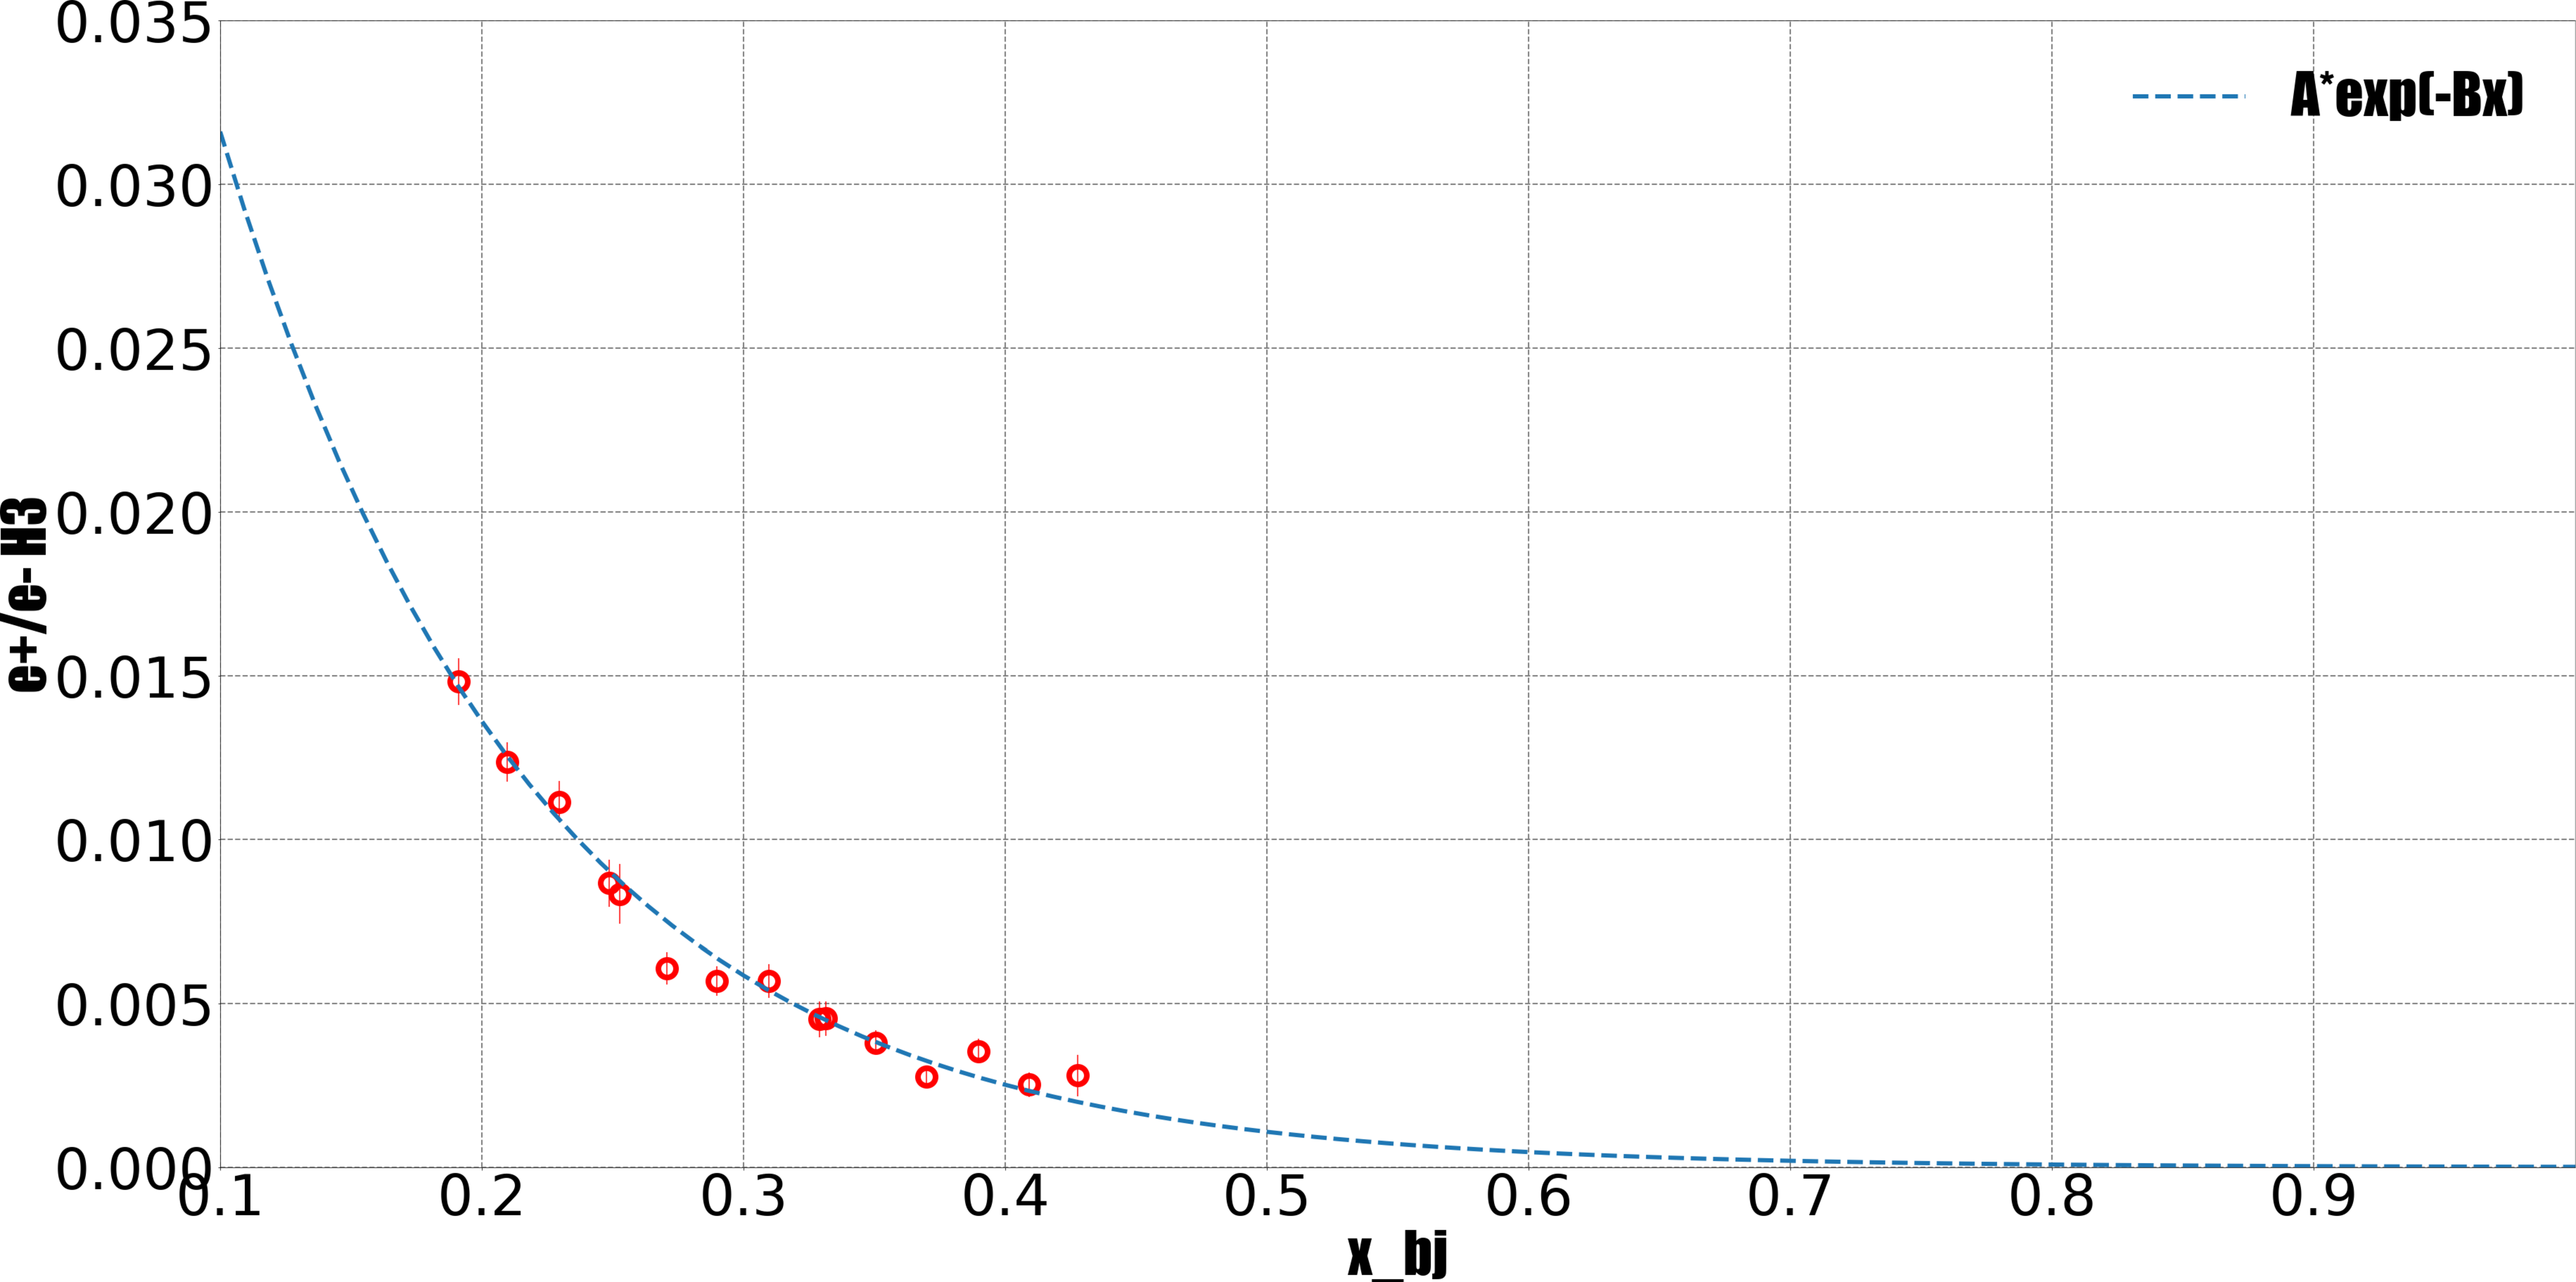
\includegraphics[width=15.0cm]{../images/positron_H3_bane.pdf}
	\caption{The ratio of positron events to electrons for tritium \cite{tongsu}. }
	\label{PC}
\end{figure}

\subsection{Beta Decay of Tritium}
\paragraph{} Tritium a radioactive isotope of hydrogen will beta decay to $^3$He. Tritium has a half-life of 4500 $\pm$ 8 days \cite{T2HL}. The gas cell used to contain Tritium for the experiment was filled on October 23, 2017. The initial tritium thickness density of our tritium cell was $0.077 \pm 0.001 $ grams per cm$^2$. Tritium will decay to $^3$He via a beta interaction. The tritium in our cell is diatomic and decays via two channels\cite{diaT}. The possible decay channels and their branching probabilities are shown in equation \ref{branching}. In DIS interactions, the molecular effects are ignored due to the size of the probe in a DIS scattering event which allows for the different channels to be treated as one. 
\begin{align}
			^3H_2 &\rightarrow(^3H ^3He)^+  &(94.5 \pm 0.6\%) \nonumber \\ 
			^3H_2 &\rightarrow(^3H)^+ + (^3He)^+  & (5.5 \pm 0.6\%) 
			\label{branching}
\end{align}
\paragraph{}The amount of $^3$H and $^3$He in our tritium cell will change in respect to the time since the feeling of the cell. Equations \ref{nT} and \ref{nH} describe the amount of $^3$H and $^3$He in the tritium cell has a function of the time since fill date and the original amount of $^3$H and $^3$He in cell at filling. In equations \ref{nT} and \ref{nH}, $n_T(n_H)$ is the time dependent amount of tritium(helium), and  $n_T^0(n_H^0)$ is the amount of tritium(helium) in the cell at time of filling. t is the time since the cell was filled and $\tau$ is the mean livetime of tritium.
\begin{align}
	n_T &= n_T^0 \: e^{-t/\tau} \label{nT}\\
	n_H &= n_H^0(1 - e^{-t/\tau}) \label{nH},
\end{align}
As time passes the amount of $^3He$ increases, the contamination becomes a non-negligible effect on the yield of scattered electrons. The fraction of $^3He$ in the tritium can reach up to 3$\%$ for the data from the end of the MARATHON experiment. This $^3He$ fraction as a function of time is shown in figure \ref{Hfract}, with the period for running the MARATHON experiment labeled as a color band. 

\begin{figure}[t]
	\centering
	\textbf{Helium Fraction from Tritium Cell. }\par\medskip
	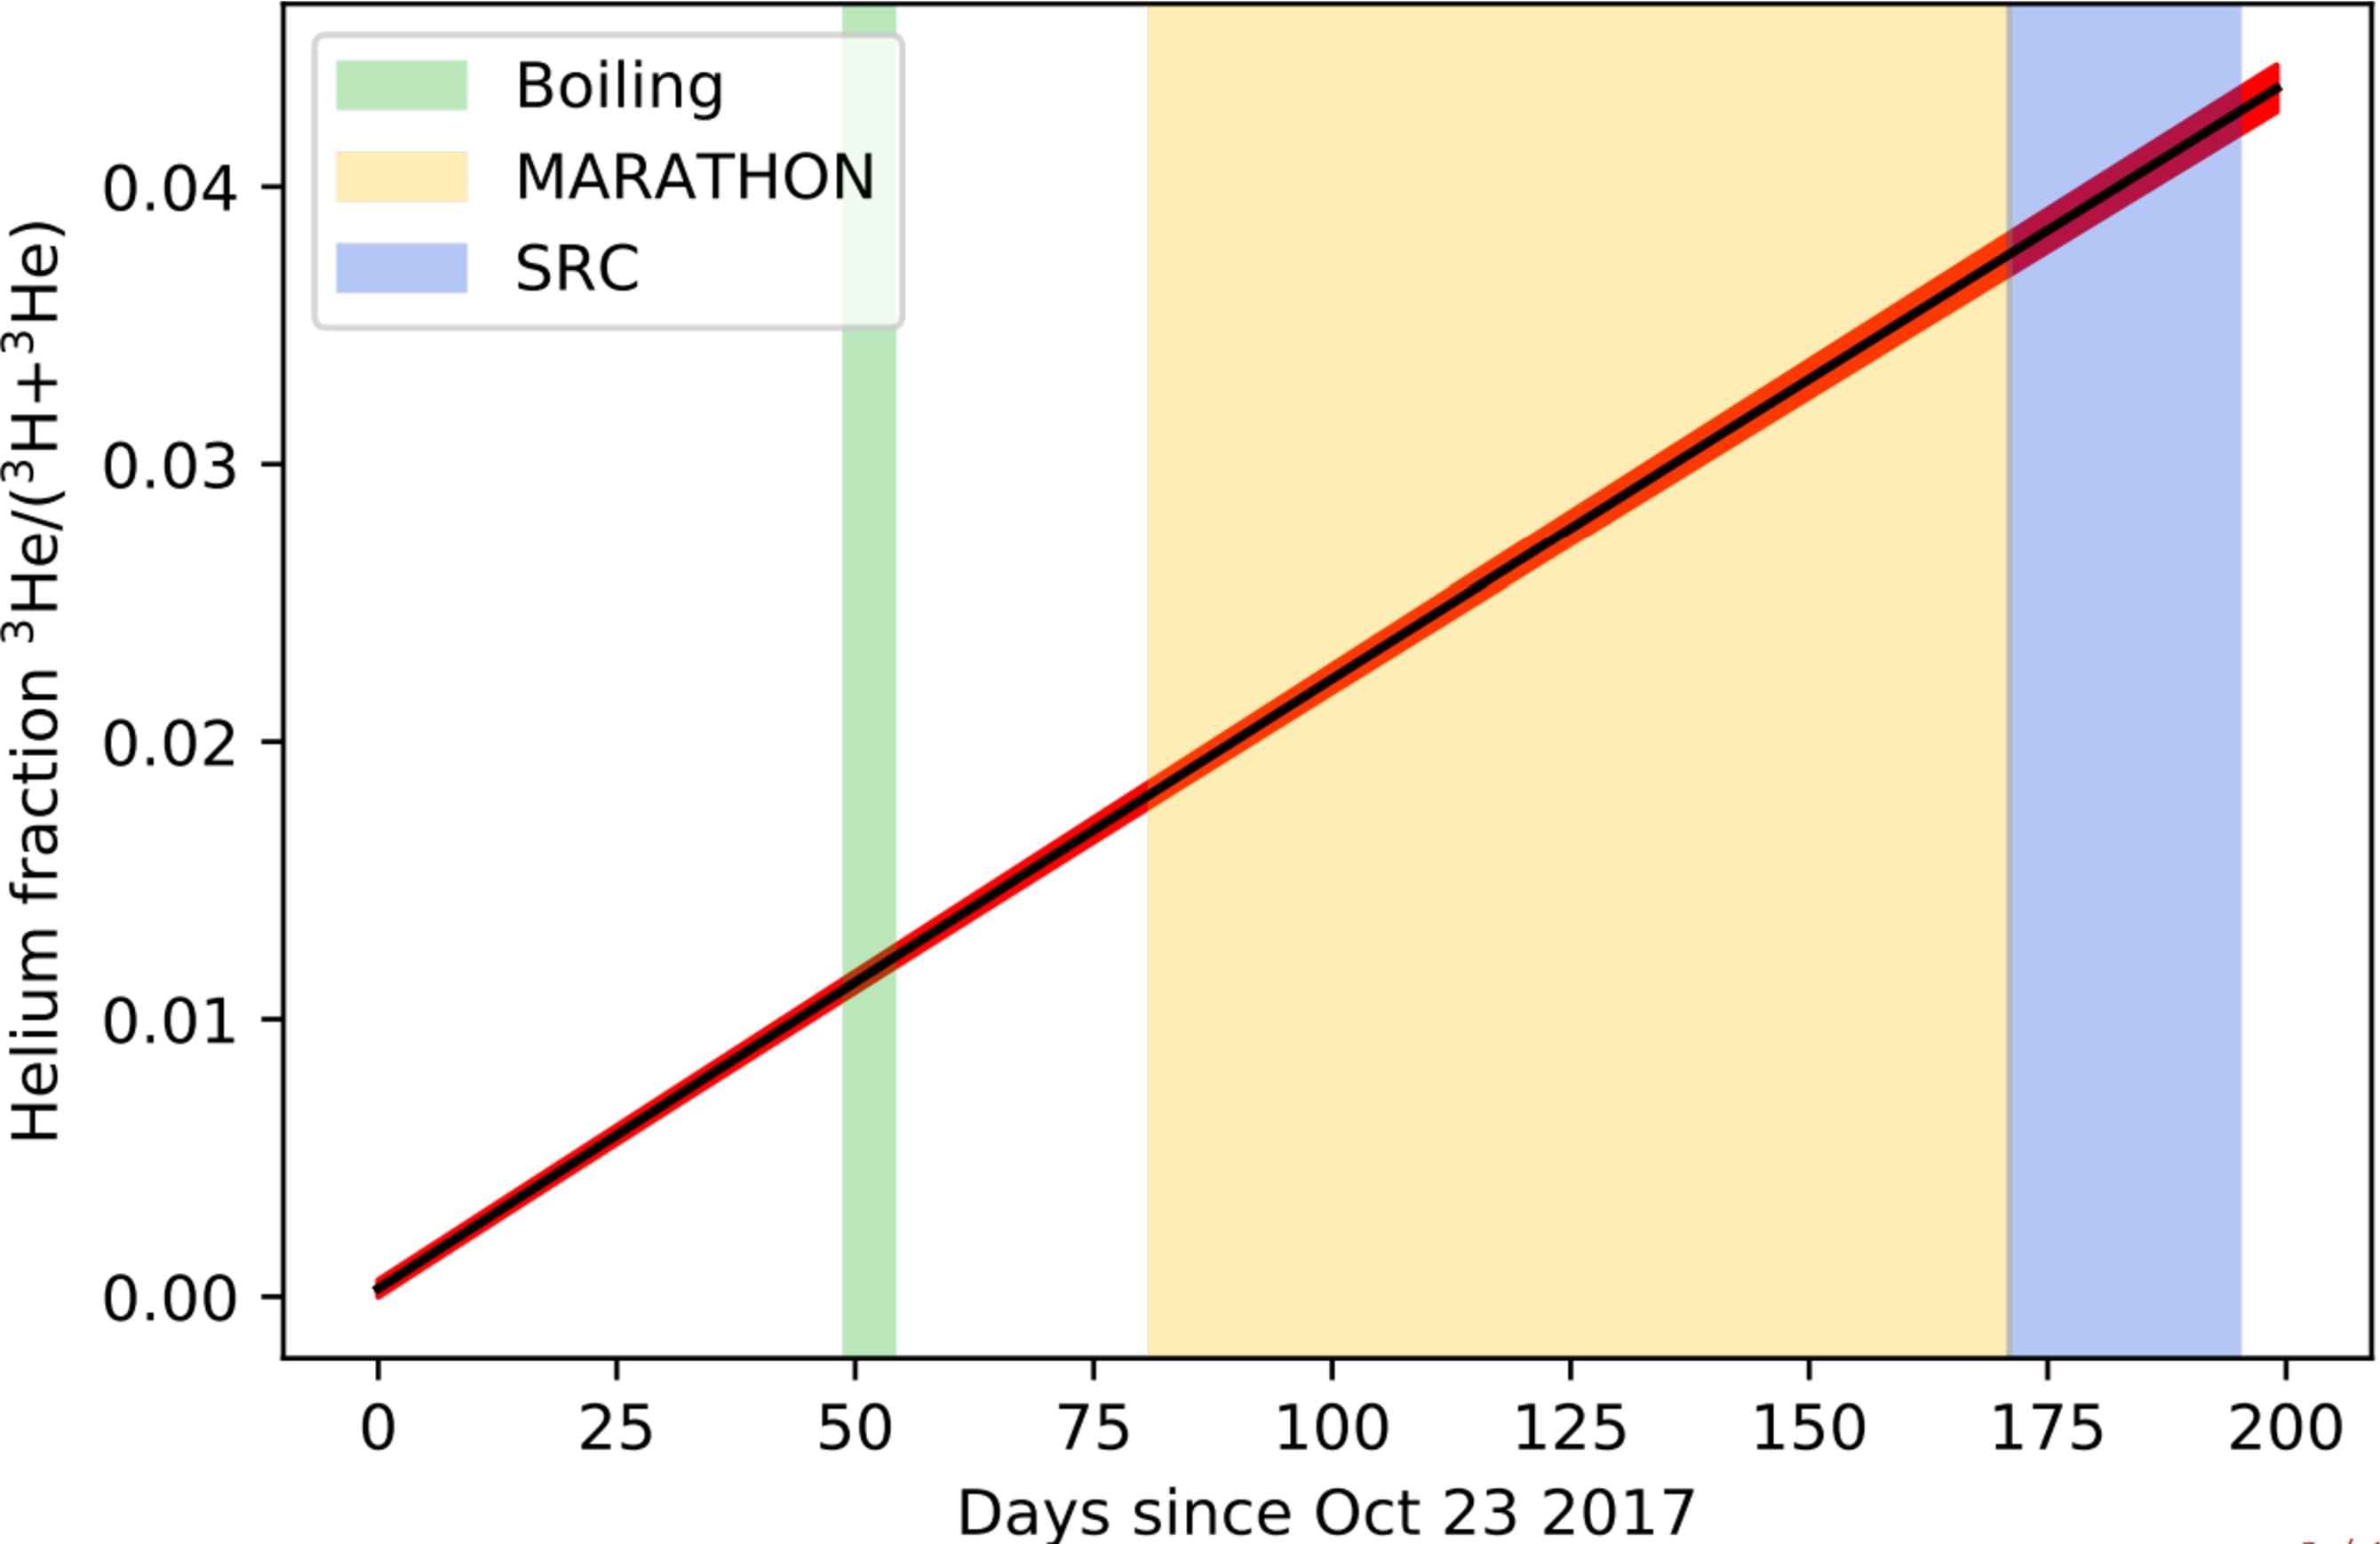
\includegraphics[width=13cm]{cont_Hfrac.pdf}
	\caption{The amount of Helium in the Tritium cell in reference to the total amount of material in the cell as a function of time. Included are bands of time for different sections of the Tritium run group's plan \cite{Beta}.}
	\label{Hfract}
\end{figure}
\begin{equation}
Y = \frac{\sum N_i}{\sum Q_i n_i}, \label{yield} 
\end{equation}
\begin{equation}
Y_{raw} = \frac{\sum (T_i + H_i)}{\sum Q_i (n_{T,i} + n_{H,i})} \label{Yraw}
\end{equation}
\begin{equation}
\langle f_H \rangle \equiv \frac{\sum Q_i f_{H,i}}{\sum Q_i} \label{QwHf}
\end{equation}


The events that scatted from Helium in our tritium cell need to be subtracted from the measured yield to supply an accurate count. The yield from any target is defined as the number of electrons per charge weighted scattering centers. The yield is shown in equation \ref{yield} and defined as the number of counted events($N_i$) per possible scattering changes, or charge($Q_i$) times number of scattering centers ($n_i$). Data is recorded in many runs, so a sum over runs($i$) is required to get the total yield. The subtraction factor is calculated by breaking down the yield from the tritium cell as the addition of the yield from tritium ($Y_T$)= $\Sigma(T_i/Q_in_{i})$ and helium ($Y_H$)= $\Sigma(H_i/Q_in_{i})$ in the tritium cell as shown in equation \ref{Yraw}. The correction for the beta decay is defined in equation \ref{YieldT}. It can be determined by expanding equation \ref{Yraw} out and solving for the tritium yield from the tritium cell. Where $\langle f_H \rangle$ is the charge weighted helium fraction defined in equation \ref{QwHf} \cite{primer}. The helium fraction $f_{H,i}$ is the ratio of helium scattering centers in the tritium cell to total number of scattering centers. 
\begin{equation}
Y_T = Y_{raw}\left(\frac{1}{1-\langle f_H \rangle}\right) - Y_H \left(\frac{\langle f_H \rangle}{1-\langle f_H \rangle}\right) \label{YieldT}
\end{equation}
The beta decay correction is applied on kinematic basis. The charge weighted average correction factor is calculated for each kinematic. The correction is then applied to the yield in each bin of that kinematic. 


\section{Luminosity}
\paragraph{}The equation of the experimentally measured cross section was shown in equation \ref{expcc}. The luminosity ($\mathscr{L}$) is the amount of possible scattering interactions. $\mathscr{L}$ is defined as the product of the number of incoming beam particles, the target particle density, and the target's thickness \cite{PnN}. The MARATHON experiment took many runs of data for each kinematic. The luminosity of each runs was calculated and summed together to determine the luminosity for each kinematic. 
\begin{equation}
	\mathscr{L}_{Run} =  \left(\frac{Q_e \cdot T_{thick} \cdot \rho_c \cdot N_a}{AtomicMass} \right) \qquad
	\mathscr{L}_{kin} = \sum_i^{Runs} \mathscr{L}_{i}
\end{equation}
The calculation of the $\mathscr{L}$ requires data from the BCMs to determine the total charge sent to the target during a run. This is converted to number of electrons to produce Q$_e$. The targets density thickness (T$_{thick}$) was provided by the JLab's target group as part of their target report \cite{HATT_eng}. Avogadro's number and the atomic mass of the target makes the luminosity have units of electrons per cm$^2$. Then applying a conversion for cm to nb gives the luminosity units commonly used for cross section extractions.
\begin{table}[]
	\caption{Table of gas target density thickness and uncertainty \cite{HATT_eng}}
	\centering
	\begin{tabular}{lcc}
	Target &Thickness(mg/cm$^2$) & Uncertainty(mg/cm$^2$)   \\
	\hline
	Tritium & 85.1 & 0.8 \\
	Helium-3 & 53.4 & 0.6\\
	Deuterium & 142.2 & 0.8\\
	\hline
	\end{tabular}
\end{table}
\paragraph{}  Due to the fluid nature of the gas targets, a target's density will fluctuate with temperature. A temperature control system uses cryogenic gas and heaters to control the temperature of the target. Power supplied to the target from the indecent beam heats the gas causing temperature fluctuations and local density variations in the target gas. A dedicated density change study was performed by S.N. Santiesteban and S. Alsalmi \cite{denscor}. Their study showed a quadric dependence on the density of the gas targets with respect to the current applied. The equation used to determine the correction applied to the target's density for a given current is shown in equation \ref{eq:dc}. Where p$_i$ are the parameters for the quadric fit, and I is the current. This correction is applied to the luminosity calculation each run by using the average current for the corresponding run. 
\begin{equation}
\rho_c = p_0 + p_1 \cdot I + p_2 \cdot I^2 \label{eq:dc}
\end{equation}
\begin{table}[]
	\caption{Table of density correction parameters \cite{denscor}.}
	\centering
	\begin{tabular}{lccc}
		Target & p$_0$ & p$_1$ & p$_2$  \\
		\hline
		Tritium & 1. $\pm$ 0.003 & (-6.8 $\pm$ 0.89) $\times 10^{-3}$ & (1.06 $\pm$ 0.36) $\times 10^{-3}$\\
		Helium-3 & 1. $\pm$ 0.003 & (-5.1 $\pm$ 0.64) $\times 10^{-3}$ & (1.04 $\pm$ 0.25) $\times 10^{-3}$\\
		Deuterium & 1. $\pm$ 0.003 & (-6.7 $\pm$ 0.71) $\times 10^{-3}$ & (1.16 $\pm$ 0.29) $\times 10^{-3}$\\
		\hline
	\end{tabular}
\end{table}

\section{Yield}
\paragraph{}The events that pass the good electron criteria are binned in bins of $x$ with varying size to decrease statistical error for the large values of $x$. The bin size ranges from 0.03 to 0.08. Events are corrected for efficiency, and background on a event by event basis. The background is accounted for through a background correction factor(BG$_i$). This factor is calculated to be a percentage of good events in the total sample and is applied as a multiplicative factor on an event basis. The efficiency ($\epsilon$) factor is a combination of the efficiency discussed in this chapter and is calculated on a run basis. The efficiencies of the current run is then applied to each good electron event. 
\begin{align}
Yield_{run}(bin) &= \sum_{i}^{\text{Good Electrons(bin)} } \left( BG_{i}/\epsilon_{i} \right) \nonumber\\
Yield_{kin}(bin) &= \sum_{run}^{runs} \bigg( Yield_{run}(bin) \bigg)
\end{align}
The yield for a kinematic is combined on a run by run basis so that the run depended corrections can be applied to the correct events. For many of the kinematics, the bins that fall within the acceptance overlap. A good electron count weighted average is used to combined the overlapping bins. 
\begin{equation}
Yield(bin) = \frac{\left( Yield_{kin}(bin)\cdot N_e^{kin}(bin)+ Yield_{kin+1}(bin)\cdot N_e^{kin+1}(bin) \right)}{N_e^{kin}(bin)+N_e^{kin+1}(bin)}
\end{equation}
\begin{figure}
	\caption{Luminosity normalized corrected yield for deuterium. The yield for each kinematic is shown as a different color and marker, with the combined yield as a grey 'x'.  \label{kinYield}}
	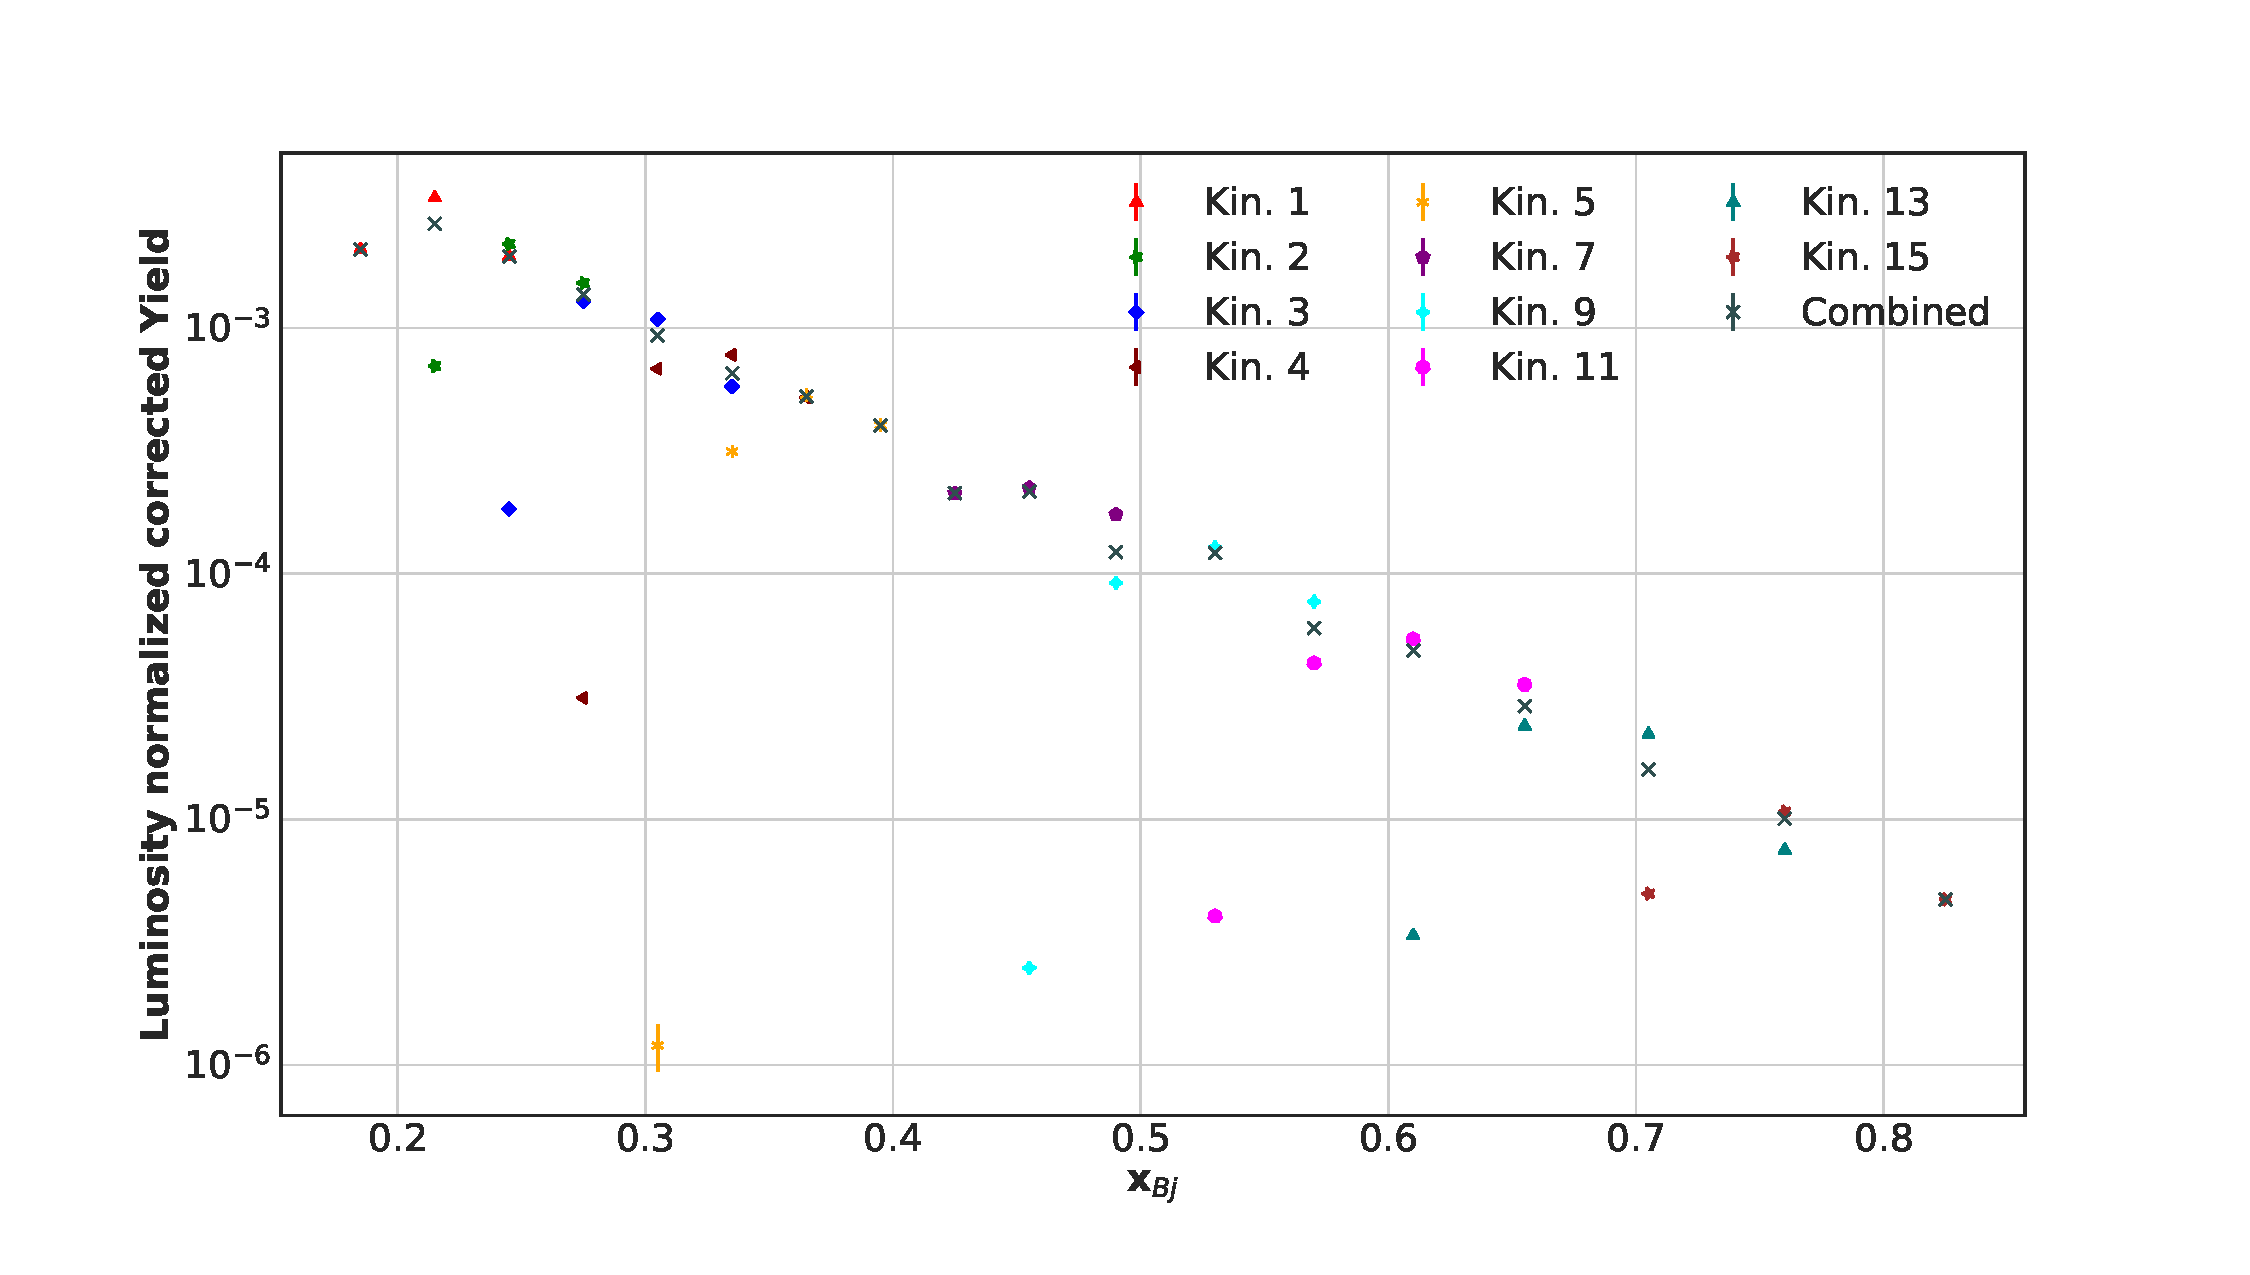
\includegraphics[width=15cm]{Yield_new.pdf}
\end{figure}
		
 \section{Monte Carlo Ratio Method}
 A Monte Carlo(MC) generated yield of electrons:
\begin{equation}
Y_{MC}(E^{\prime},\theta) = \mathscr{L} \cdot \sigma^{model} \cdot (\Delta E^{\prime} \Delta \Omega) \cdot A(E^{\prime},\theta)
\end{equation}
Rewriting the MC generated yield to emphasize the normalization factors, luminosity, phase space and acceptance allows for a direct comparison with the experimental cross section using the measured yield.
\begin{align}
Y_{MC}(x) / \sigma^{model} &= \mathscr{L} \cdot (\Delta E^{\prime}_{MC} \Delta \Omega_{MC}) \cdot A(E^{\prime},\theta)_{MC} \\
\sigma^{data}(x) &= \frac{Y_{data}(x)}{ \mathscr{L} \cdot (\Delta E^{\prime}_{Data} \Delta \Omega_{Data}) \cdot A(E^{\prime},\theta)_{Data} }
\end{align}

\paragraph{} The acceptance for a bin, A($E^{\prime},\theta$), is defined as the probability that a particle of energy $E^{\prime}$ and scatted angle $\theta$ will be able to pass through the spectrometer. This analysis will use a Monte Carlo(MC) simulation to account for the acceptance of the HRS in a bin of $x$.

This analysis uses the hall A single arm Monte carlo simulation to simulate events so that A$_{MC}$ is equivalent to A$_{Data}$. Using the monte carlo ratio method, the experimental cross section can be calulated for a bin of $x$ by:
\begin{equation}
\sigma_{Data} = \sigma_{model} \cdot \frac{Y_{Data}}{Y_{MC}}.
\end{equation} 
This section will discuss the Monte Carlo simulation and compare the yield of Monte Carlo to the yield from data.

\subsection{Monte Carlo Simulation}

\paragraph{}The process of creating MC yields contains three steps: 
\begin{itemize}
	\item production of cross section table with radiative corrections
	\item event generation,
	\item weighing accepted events with the model cross section .
\end{itemize} 
\subsubsection{Cross Section Table}
\vspace{-10pt}\paragraph{} A cross section model is used to weight the Monte Carlo events to make a comparison between a Monte Carlo yield and a yield from data. The Born cross section is calculated via a DIS model with an EMC model correction. An Arie Bodek model \cite{DISmodel} is used to determine the nuclear structure function in the DIS regime. This same model uses a smearing technique to include any effects from the elastic and quasi-elastic tail. The kinematics closest to the resonance region experiences an almost negligible quasi-elastic contribution. A correction calculated from SLAC EMC data is applied to correct for the building of the nuclear structure function from free nucleon structure functions. The resulting born cross section is used to weigh events in the Monte Carlo simulation. Figure \ref{MCS} shows the born cross section for tritium at kinematic 1 for scattered angle along the x-axis and scattered momentum along the z-axis associated with color.  

\begin{figure}
	\caption{Model cross section for tritium at kinematic 1 for scattered angle and momentum. \label{MCS}}
	\hspace{-40pt}
	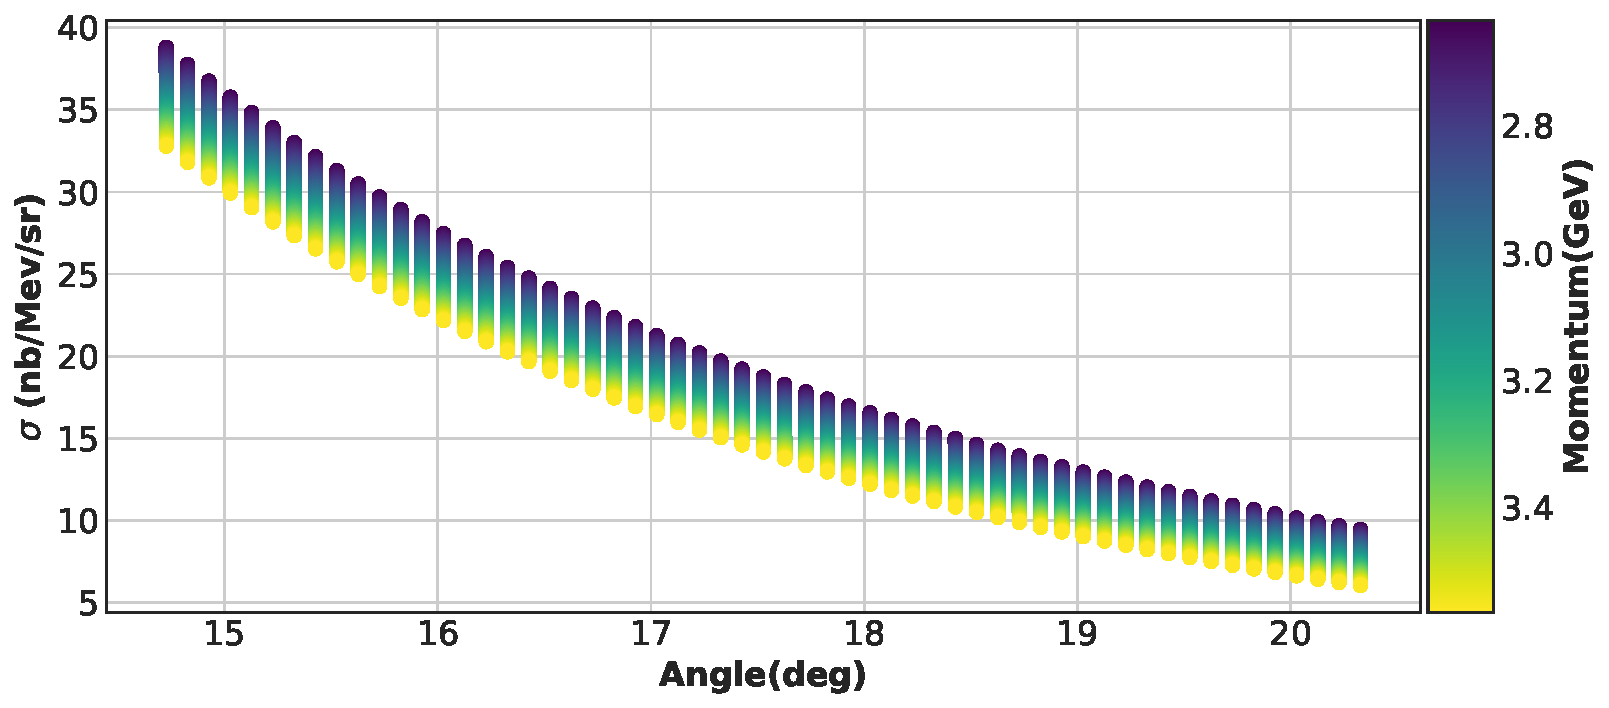
\includegraphics[width=18cm]{cs_m_T1.pdf}
\end{figure}
\paragraph{} The scattered event that is measured through the experiment is not alone the Born process (the one photon exchange approximation) shown in figure \ref{fig:radcors} but a combination of all the other processes shown. In order to produce a comparable result with data, these higher order contributions have to be addressed.
\begin{figure}[h]
	\centering
	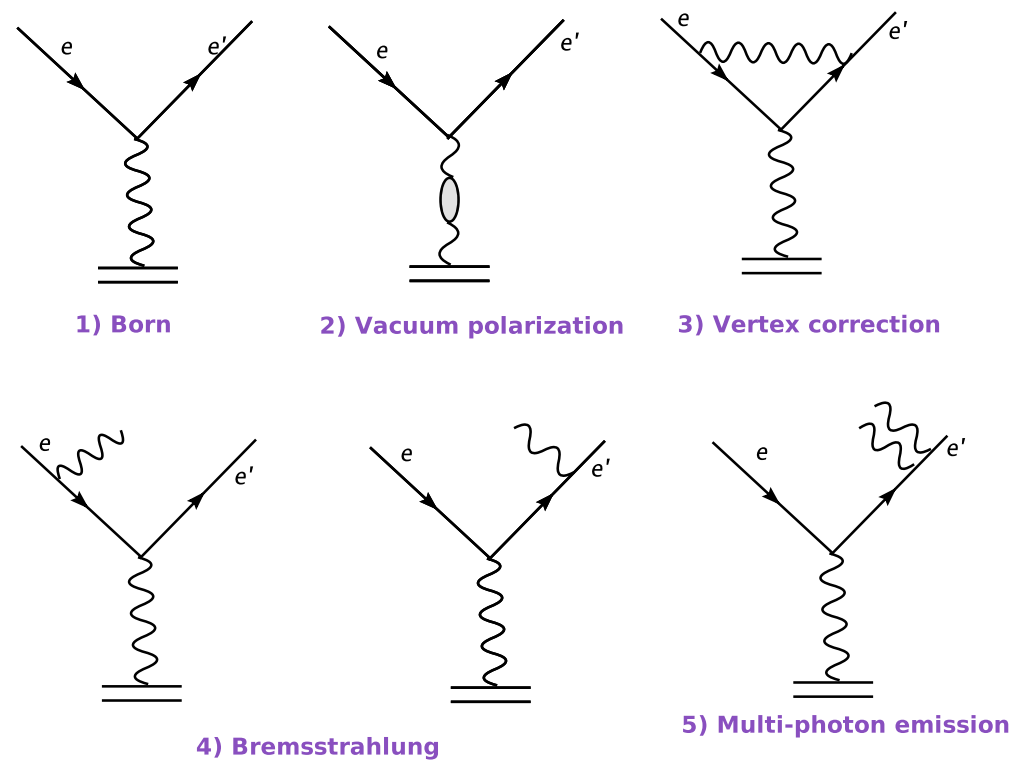
\includegraphics[width=10cm]{radcors.png}
	\caption{Lowest order Feynman diagrams for inclusive lepton-nucleon scattering \cite{Ajth}.}
	\label{fig:radcors}
\end{figure} 
\paragraph{}There are two broad types of radiative effects that needed be account for during an electron nucleus scattering interaction, internal and external. External effects account for the electron radiating a real photon before or after the designated target. This radiation is caused by an interaction with fields of nuclei that make up the material other then the target. External bremsstrahlung and ionization energy losses are two of the process that occur causing these external effects. The internal radiative effects happen at the interaction point, the scattering vertex. The Feynman diagrams in figure \ref{fig:radcors} shows the lowest order approximation for the possible interaction channels. These high order processes are calculable in QED. Mo and Tsai \cite{radcors2} and S. Sasu \cite{radcors} describe in detailed the method of calculating these radiative effects. This analysis used a radiative correction code originally by S. Dasu \cite{radcors}. This package use Mo and Tsai's formula to complete the measured cross section calculation.  The internal bremsstrahlung contribution is calculated via an equivalent radiator approximation. A full integral calculation is done over the entire length of radiators to make a complete calculation for the entire radiative effect  \cite{Ajth,radcors,radcors2,seelyth}. A correction is applied as a weighing factor with the born cross section. A 2 dimensional grid is made from a scan of possible scatted angles covering the acceptance of the spectrometer for each value of scatted momentum possible for the kinematic setting. This grid is then used to populate a cross section table for each target at each kinematic. The cross section and radiative correction factor are calculated for the combination of kinematic variables to complete the cross section table(CST). Figure \ref{RCF} shows the radiative correction factor ($RCF=\frac{\sigma_{Rad}}{\sigma_{Born}}$) for tritium at kinematic 1 for scattered angle along the x-axis and scattered momentum along the z-axis associated with color.  
\begin{figure}
	\caption{Radiative correction for Tritium at kinematic 1, for scattered angle and momentum.\label{RCF}}
	\hspace{-40pt}
	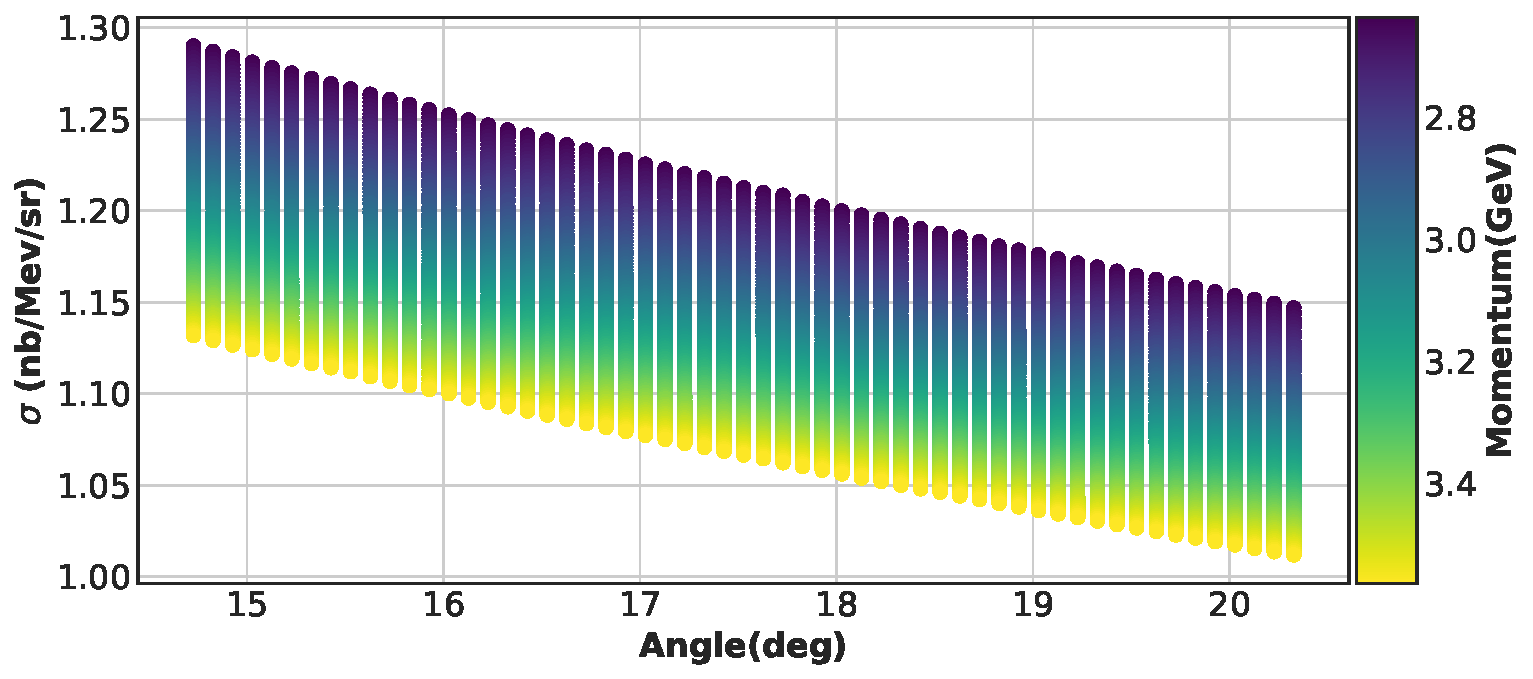
\includegraphics[width=18cm]{rad_m_T1.pdf}
\end{figure}

\subsubsection{Generation}
\paragraph{}The MC simulation generates events in the target frame to travel from the point of interaction to the spectrometer's focal plane. The events are generated to have a uniform distribution in $\delta$, $\theta$, and $\phi$. A generated event drifts from the randomized point of interaction to the entrance of the spectrometer. Along this drift, the simulation calculates the chances of multiple scattering events using the radiation length of the intervening material. Simulated electrons pass through the remaining target length, aluminum endcap, vacuum, aluminum wall of the scattering chamber, air, and kapton film at the entrance of the spectrometer's vacuum. Once entering the spectrometer, the simulated event will use differential algebra based COSY model to pass through the magnetic field of the spectrometer's dipole and quadrapoles. The code checks a particles trajectory through the spectrometer ensuring no collision with the magnetic apertures.  Events that have successfully traveled to the VDC will receive a smearing effect to account for the finite resolution of the VDCs in the HRS \cite{HallA}. The event's focal plane coordinates are used to transform back to the target coordinates to calculate the scattered energy and scattered angle.\\ 
\subsubsection{Event Weighting}
\paragraph{}An accepted Monte Carlo event is weighted to best match physical conditions. The comparison of simulation with actual data requires the event to be weighted with the born cross section of that event and corrected for radiative effects. The subroutine used for this analysis uses a 2 dimensional interpolation (scattered energy and momentum) to determine the born cross section and radiative correction factor for the exact event. The 2D interpolation is completed by finding 4 locations on the cross section table. For the following description of the table locations, $_{evt} =$ event and $_{cst} =$ cross section table. The cross section value is pulled from the table for a row that meets the criteria. For example, $\sigma[1]$ is the born cross section for the row where the angle is closest but lower then the event and the momentum is closest but lower then the event. 
\begin{align}
 	\sigma[1] &=\sigma[\theta_<][P_<]\rightarrow\,(P^{\prime}_{cst}\, <=\, P^{\prime}_{evt}\; \&\& \;\theta_{cst}\, <=\, \theta_{evt}) \nonumber\\
	\sigma[2] &=\sigma[\theta_<][P_>]\rightarrow\,(P^{\prime}_{cst}\, >=\, P^{\prime}_{evt}\; \&\& \;\theta_{cst}\, <=\, \theta_{evt}) \nonumber\\
	\sigma[3] &=\sigma[\theta_>][P_<]\rightarrow\,(P^{\prime}_{cst}\, <=\, P^{\prime}_{evt}\; \&\& \;\theta_{cst}\, >=\, \theta_{evt}) \nonumber\\
	\sigma[4] &=\sigma[\theta_>][P_>]\rightarrow\,(P^{\prime}_{cst}\, >=\, P^{\prime}_{evt}\; \&\& \;\theta_{cst}\, >=\, \theta_{evt})
\end{align}
Each cross section value has it's corresponding momentum $P[i]$, angle $\theta[i]$, and the momentum and angle differences between the event and table  $\Delta P[i]$, and $\Delta \theta[i]$. The 2D interpolation is broken down into two 1D interpolations between the momentum values.
\begin{align}
\sigma_1 &= \frac{\left(\sigma[1] \cdot \Delta P[1] +  \sigma[2] \cdot \Delta P[2] \right)} {P[2]-P[1]}\nonumber\\
\sigma_2 &= \frac{\left(\sigma[3] \cdot \Delta P[3] +  \sigma[4] \cdot \Delta P[4] \right)} {P[4]-P[3]}
\end{align}
Then an interpolation is done between the calculated $\theta$ values.
\begin{equation}
\sigma = \frac{\left(sigma_2 \cdot \Delta \theta[3] + sigma_1 \cdot \Delta \theta[1]\right) }{\theta[3] -\theta[1]}
\end{equation}
The 2D interpolation is completed both for the born cross section and the radiative correction factor for each accepted simulated event.
\subsection{Monte Carlo Comparison}
\paragraph{}The weighted Monte Carlo events are binned into the target and focal planes for comparison to data. The comparison is used to determine the quality of the simulation. Figure \ref{tcomp} and \ref{fcomp} show the comparison for target plane variables and focal plane variables respectively. The important target variables to study are $\delta_{tg}$, y$_{tg}$, out of plane angle($\theta_{tg}$), and the in plane angle($\phi_{tg}$). 
\begin{figure}[h]
	\caption{Monte Carlo to Data comparison for target plane variables, top left $\delta$ ,bottom left y, top right $\theta$, bottom right $\phi$. Run 1207, kinematic 1 on carbon foil.\label{tcomp}}
	{\centering
	\hspace{-50pt}
	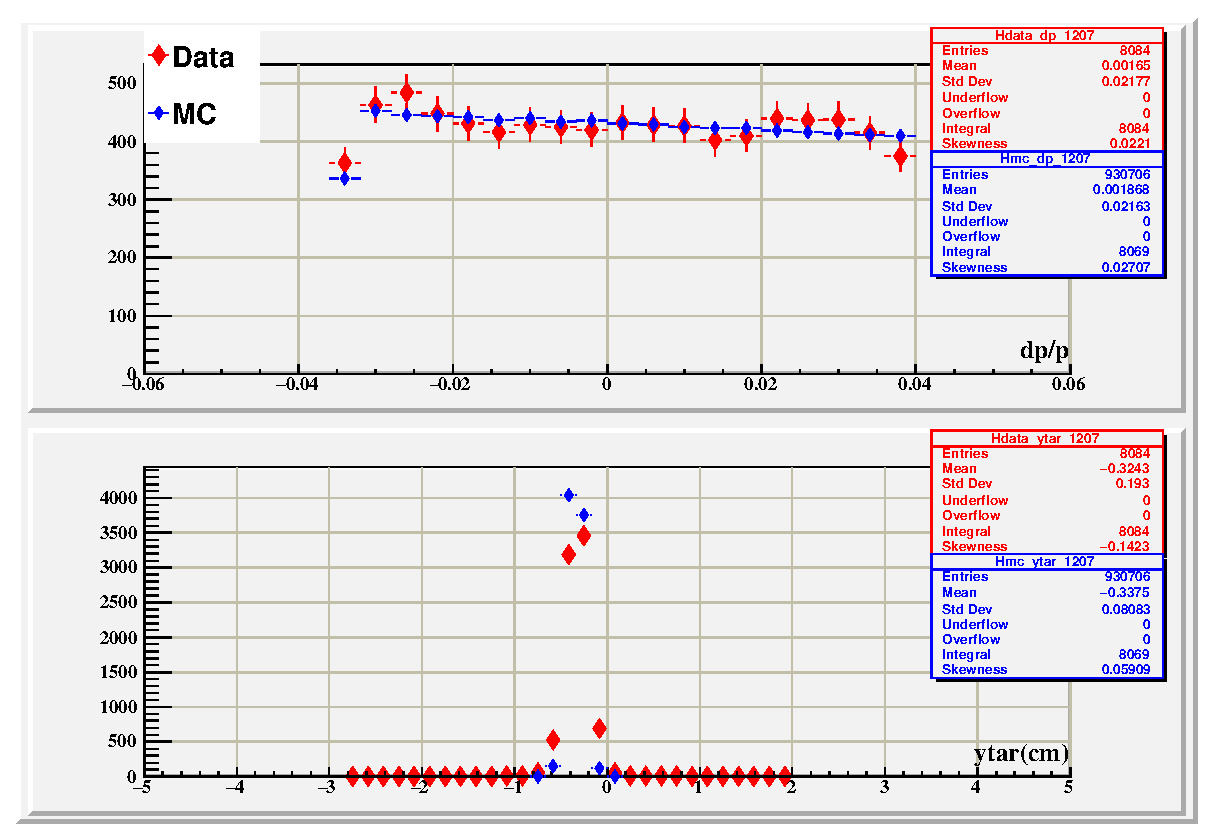
\includegraphics[height=7.5cm,width=9cm]{dp_ytar_1207.eps}
	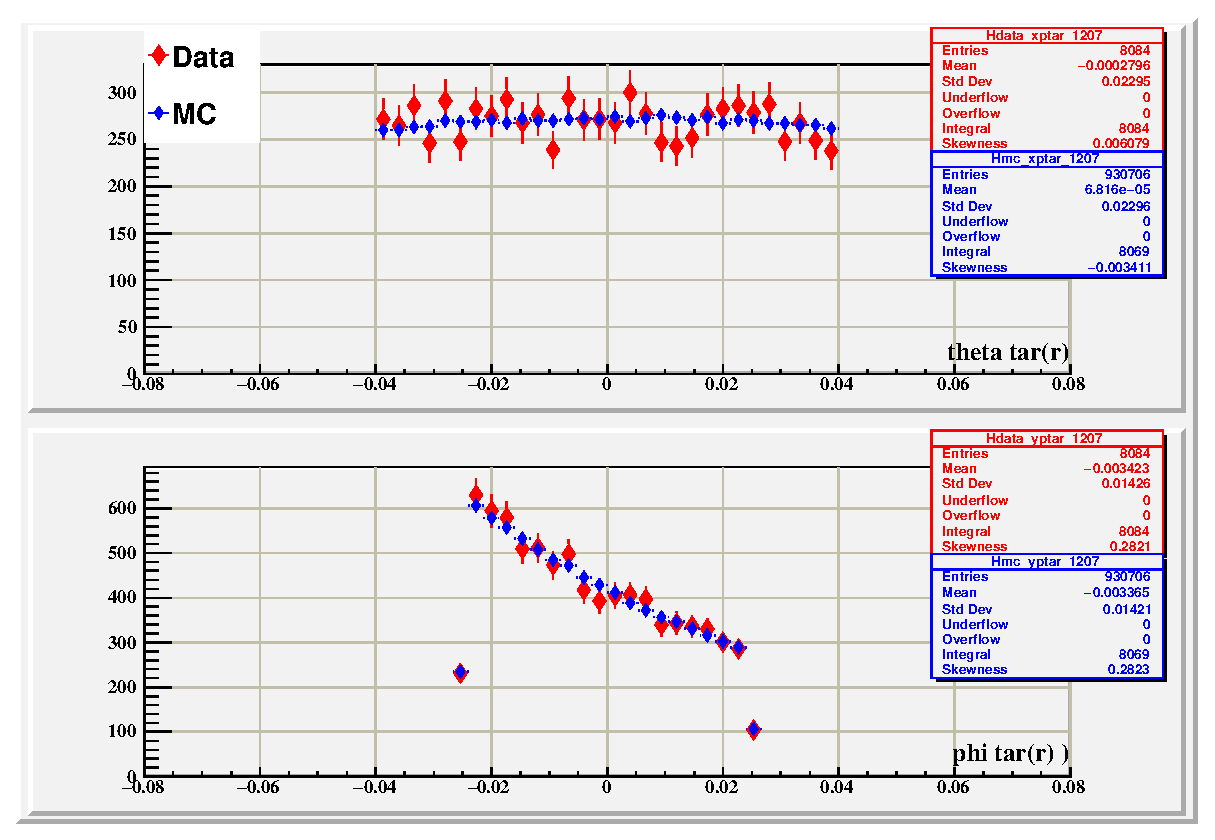
\includegraphics[height=7.5cm,width=9cm]{xp_yp_tar_1207.eps}
}
\end{figure}
\begin{figure}[H]
	\caption{Monte Carlo to Data comparison for focal plane variables, top left $\theta$ ,bottom left $\phi$, top right $x$, bottom right $y$. Run 1207, kinematic 1 on carbon foil. \label{fcomp} }
	{\centering
	\hspace{-50pt}
	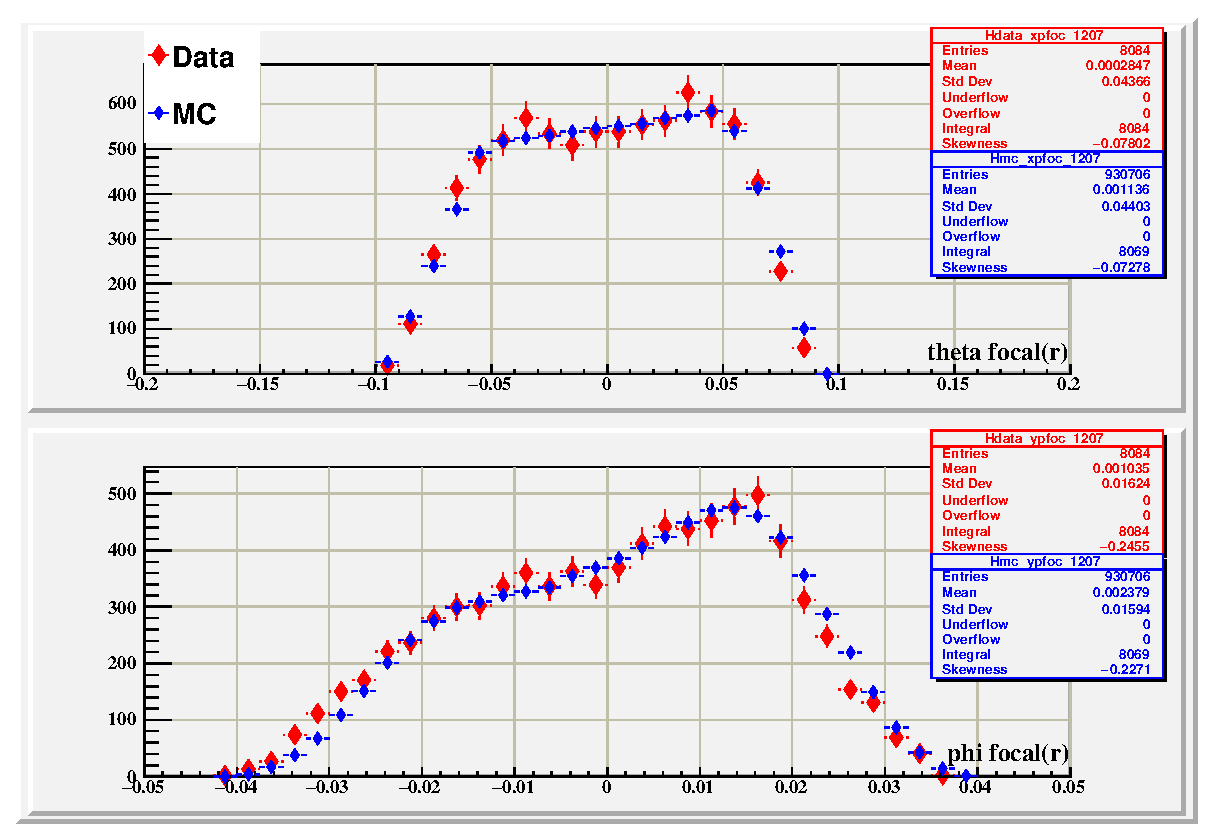
\includegraphics[height=7.5cm,width=9cm]{xp_yp_foc_1207.eps}
	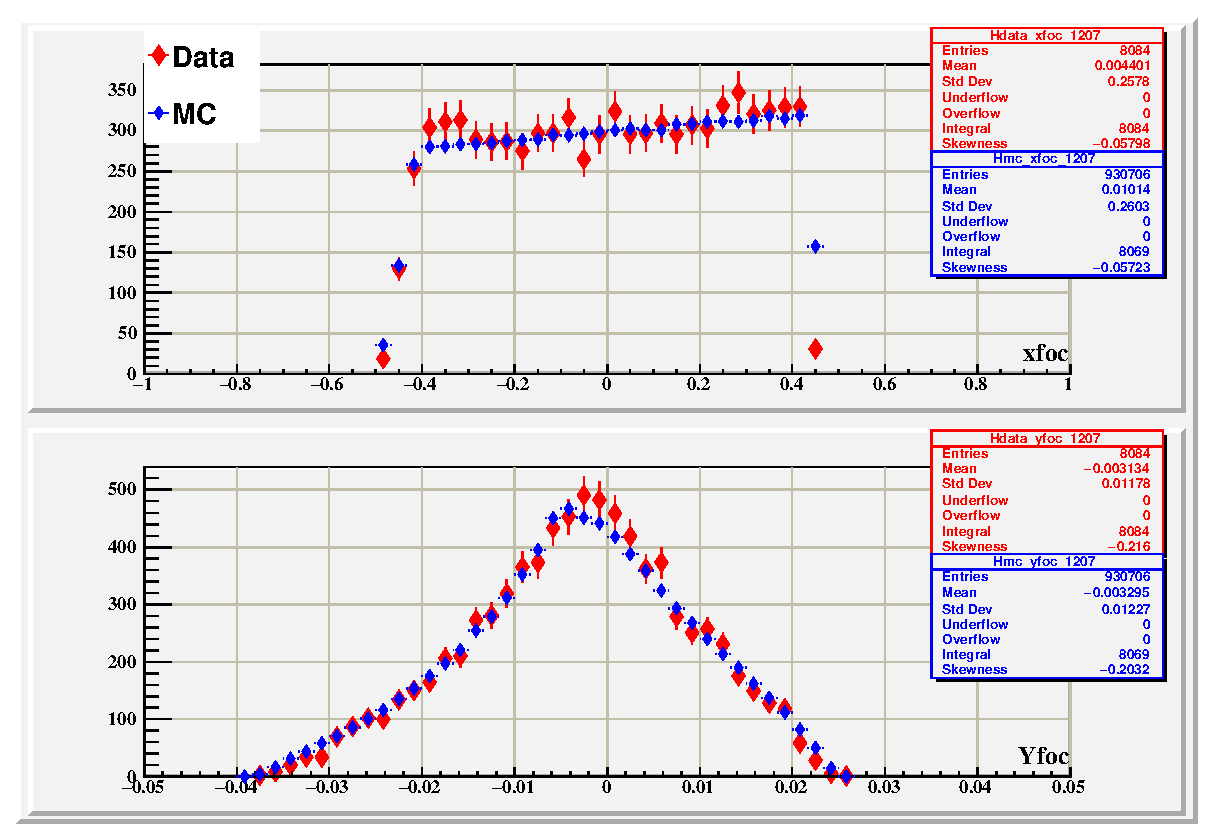
\includegraphics[height=7.5cm,width=9cm]{x_y_foc_1207.eps}}
\end{figure}
The yield dependence in $\phi_{tg}$ and $\delta_{tg}$ are expected due to the dependence of the cross section on those variables. The good comparison for those quantities show the simulation's good performance in matching the spectrometers acceptance and the cross section models functional form. The comparison between data and Monte Carlo has been deemed good, with 99\% comparison for the single foil carbon target. 

\section{DIS Cross Section}
\paragraph{}Using the Monte Carlo ratio method, I extracted the experimental measured cross section for helium-3, tritium, and deuterium. These DIS cross section extraction ranges from 0.18 to 0.82 in $x$, from 2.2 to 11.8 GeV$^2$ in $Q^2$, and has W$^2$ $>3.5$ GeV$^2$. 

\begin{equation}
\sigma_{Data} = \sigma_{model} \cdot \frac{Y_{Data}}{Y_{MC}}. \nonumber
\end{equation} 

\begin{figure}
	\caption{Comparison of the yield of Data to Monte Carlo for deuterium in bins of $x$ for each kinematic. \label{d-mc comp}}
	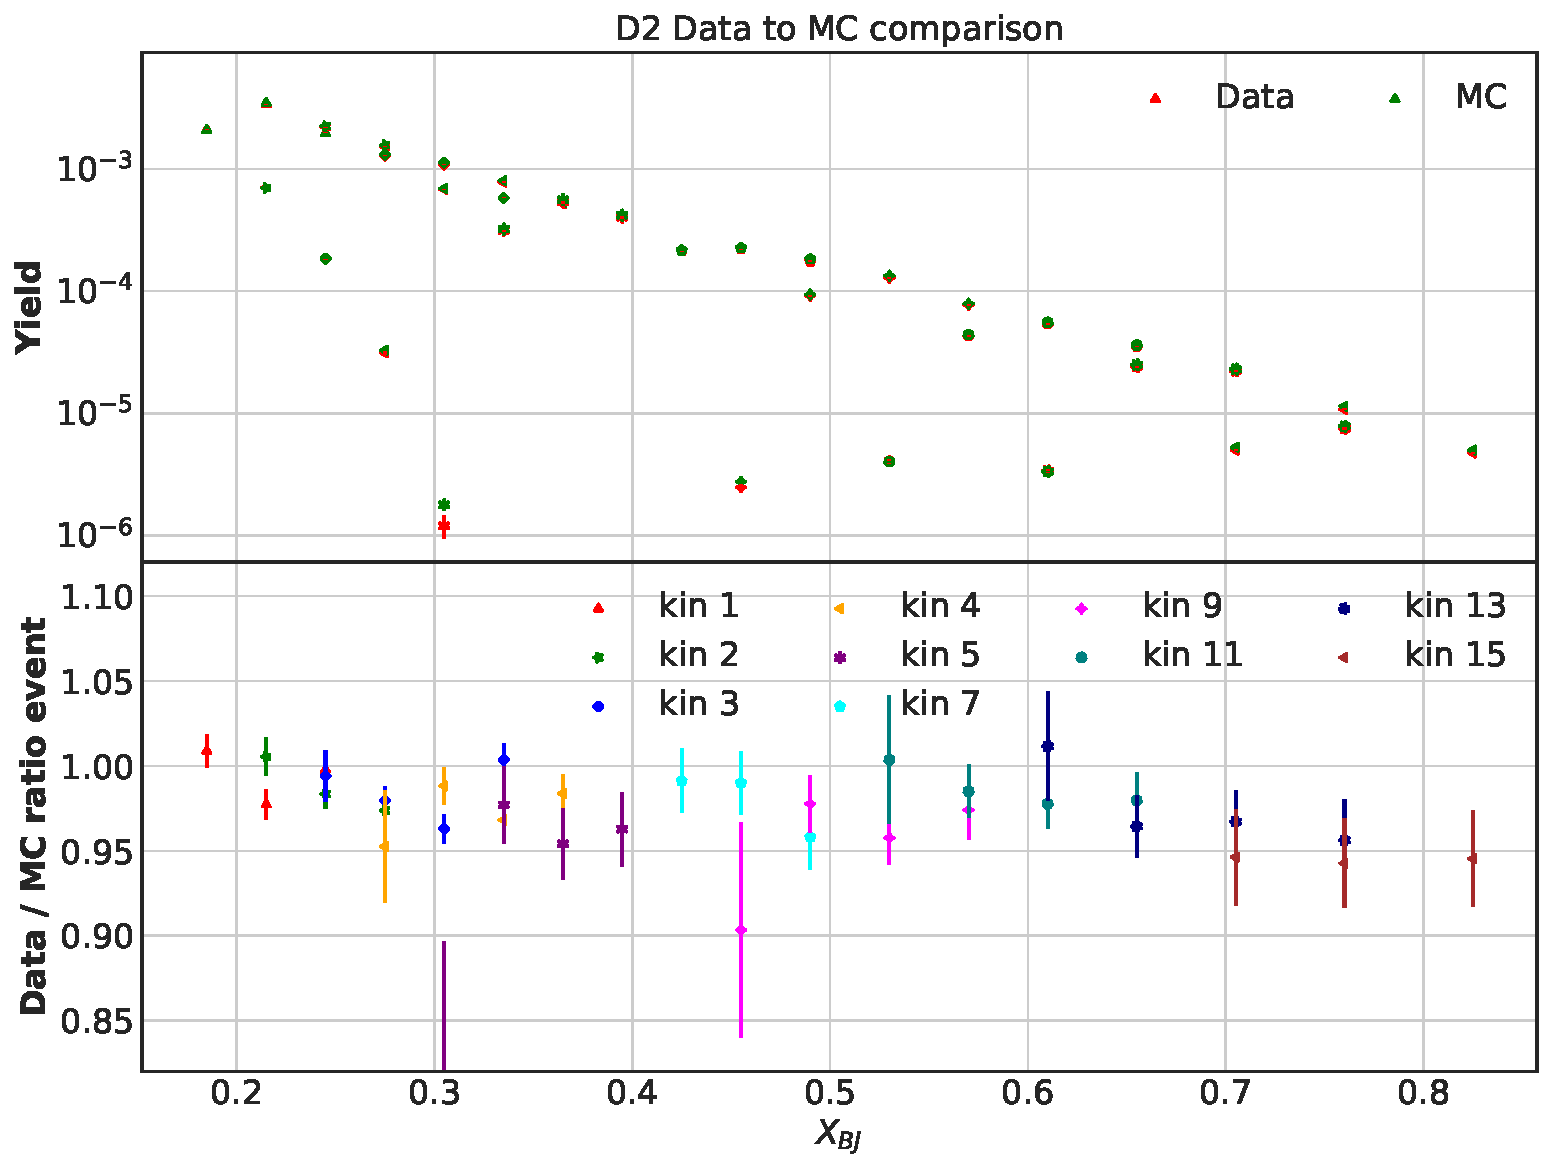
\includegraphics[width=15cm]{YieldComp.pdf}
\end{figure}
\paragraph{}Using the ratio of the yield from data to the yield from Monte Carlo, I manipulate the model cross section to calculate the experimentally measured cross section.
 
\begin{figure}
	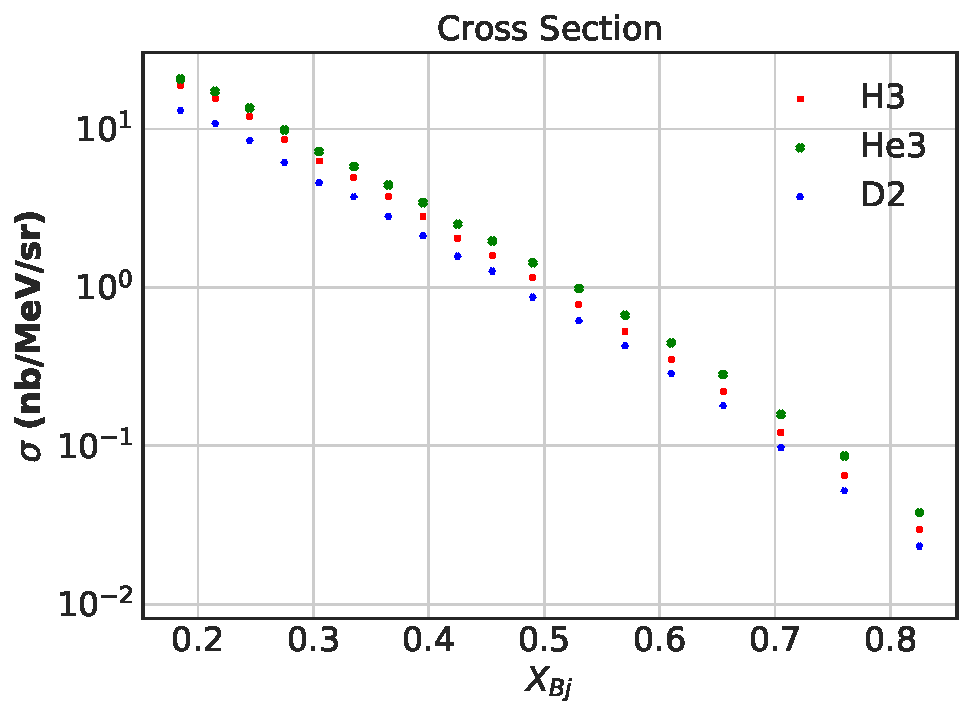
\includegraphics[width=15cm]{total_xs.pdf}
	\caption{Experimentally measured cross section using the Monte Carlo ratio method for tritium, helium-3, and deuterium. Normalization uncertainty due to target thickness uncertainty for tritium= 0.97\%, helium-3 = 1.12\%, and deuterium = 0.56\%. }

\end{figure}

\section{Systematic Error}
\cite{Ar_Ti}




